\documentclass[10pt]{beamer}
\usetheme[
%%% option passed to the outer theme
%    progressstyle=fixedCircCnt,   % fixedCircCnt, movingCircCnt (moving is deault)
  ]{Feather}
  
% If you want to change the colors of the various elements in the theme, edit and uncomment the following lines
\definecolor{grey}{rgb}{0.52, 0.52, 0.51}

% Change the bar colors:
\setbeamercolor{Feather}{fg=grey!20,bg=grey}
% This is the inner theme file of the Feather theme.
% Copyright (c) 2014 by Lilyana Vaskova Vankova <lilqna.v@gmail.com>
%
% This program is free software: you can redistribute it and/or modify
% it under the terms of the GNU General Public License as published by
% the Free Software Foundation, either version 3 of the License, or
% (at your option) any later version.
%
% This program is distributed in the hope that it will be useful,
% but WITHOUT ANY WARRANTY; without even the implied warranty of
% MERCHANTABILITY or FITNESS FOR A PARTICULAR PURPOSE.  See the
% GNU General Public License for more details.
%
% You can find the GNU General Public License at <http://www.gnu.org/licenses/>.

%----------------------------------------------------------------------------------------------------------------------------------

\NeedsTeXFormat{LaTeX2e}
\ProvidesPackage{beamerinnerthemeFeather}[2014/04/08 v1.0.0 The Feather Beamer Theme]

%----------------------------------------------------------------------------------------------------------------------------------

%%%%%%%%%%%%%%%%%%%%%%%%%%%%%%%%%%%%%%%%%%%%%%%%
% Theme options, definitions and templates.
%%%%%%%%%%%%%%%%%%%%%%%%%%%%%%%%%%%%%%%%%%%%%%%%

%----------------------------------------------------------------------------------------------------------------------------------

% beamer specific options

               \mode<presentation> %refers to the first four modes (beamer,handout,second and trans). That is, to all modes except the article mode
{

%----------------------------------------------------------------------------------------------------------------------------------

% title page
%% definitions for fonts of the different elements
  
               \setbeamerfont{institute}{family=\rmfamily, size = \footnotesize}
               \setbeamerfont{title}{family=\rmfamily, size = \huge} 
               \setbeamerfont{subtitle}{family=\rmfamily, size = \Large}
               \setbeamerfont{author}{family=\rmfamily, size = \footnotesize}
               \setbeamerfont{date}{family=\rmfamily, size = \footnotesize}

               \setbeamertemplate{title page}
   {

%% setting the above definitions

        \begin{minipage}[c][\textheight][c]{\textwidth}

                  \centering

                 {\usebeamerfont{institute}\insertinstitute}\vspace*{30pt}

                 {\usebeamerfont{title}\usebeamercolor[fg]{title}\inserttitle}\vspace*{10pt}

                 {\usebeamerfont{subtitle}\usebeamercolor[fg]{subtitle}\insertsubtitle}\vspace*{30pt}

                 {\usebeamerfont{author}\insertauthor}\vspace*{30pt}

                 {\usebeamerfont{date}\insertdate}\vspace*{\baselineskip}

         \end{minipage}
   }
  
%----------------------------------------------------------------------------------------------------------------------------------
  
% final page

                  \defbeamertemplate{final page}{text}[1]
   {
         \begin{minipage}[c][\textheight][c]{\textwidth}
                  \centering
                  #1
         \end{minipage}
   }
                  \newcommand{\finalpage}[1]
   {
                  \setbeamertemplate{final page}[text]{#1}
                  \usebeamertemplate{final page}
   }

%----------------------------------------------------------------------------------------------------------------------------------
  
% add the feather to the background of the titlepage and the final page

                  \newcommand{\1}
   {
                  \setbeamertemplate{background}
      {
                  
\includegraphics[height=\paperheight]{Feathergraphics/1}
                  \tikz[overlay] \fill[fill opacity=0.8,fill=white] (0,0) rectangle (-\paperwidth,\paperheight);
       }
    }

%----------------------------------------------------------------------------------------------------------------------------------
  
% use numbers instead of a picture for the references

                  \setbeamertemplate{bibliography item}[text]

}

\mode<all>
% Change the color of the structural elements:
\setbeamercolor{structure}{fg=grey}

% Change the frame title text color:
%\setbeamercolor{frametitle}{fg=blue}

% Change the normal text color background:
\setbeamercolor{normal text}{fg=black,bg=gray!10}

%-------------------------------------------------------
% INCLUDE PACKAGES
%-------------------------------------------------------

\usepackage[utf8]{inputenc}
\usepackage[english]{babel}
\usepackage[T1]{fontenc}
\usepackage{helvet}
\usepackage{lipsum}
\usepackage{tikz}


%-------------------------------------------------------
% DEFFINING AND REDEFINING COMMANDS
%-------------------------------------------------------

% colored hyperlinks
\newcommand{\chref}[2]{
  \href{#1}{{\usebeamercolor[bg]{Feather}#2}}
}

%-------------------------------------------------------
% INFORMATION IN THE TITLE PAGE
%-------------------------------------------------------

\title[] % [] is optional - is placed on the bottom of the sidebar on every slide
{ % is placed on the title page
      \textbf{Wavelength}
}

\subtitle[$\lambda$-IDE]
{
      \textbf{$\lambda$-IDE}
}

\author[wavelength]
{      Muhammet Guemues \\
       Markus Himmel \\
       Marc Huisinga \\
       Philip Klemens \\ 
       Julia Schmid \\  
       Jean-Pierre von der Heydt \\     
}

\institute[]
{
      
  
  %there must be an empty line above this line - otherwise some unwanted space is added between the university and the country (I do not know why;( )
}

\date{30.11.2017}

%-------------------------------------------------------
% THE BODY OF THE PRESENTATION
%-------------------------------------------------------

\begin{document}

%-------------------------------------------------------
% THE TITLEPAGE
%-------------------------------------------------------

%{\1 % this is the name of the PDF file for the background
% Mein PDF-Viewer bekommt das nicht hin, das Bild im Hintergrund anzuzeigen
{
%\setbeamertemplate{background canvas}{\tikz[remember picture,overlay]\node[opacity=0.3] at (current page.center) {
\includegraphics[height=\paperheight]{img/Logo.pdf}};}
\begin{frame}[plain]
\maketitle
\end{frame}
}
%}


%\begin{frame}{Content}{}
%\tableofcontents
%\end{frame}

\begin{frame}[plain,noframenumbering]

\begin{overlayarea}{\textwidth}{\textheight}
\begin{figure}
    \only<1>{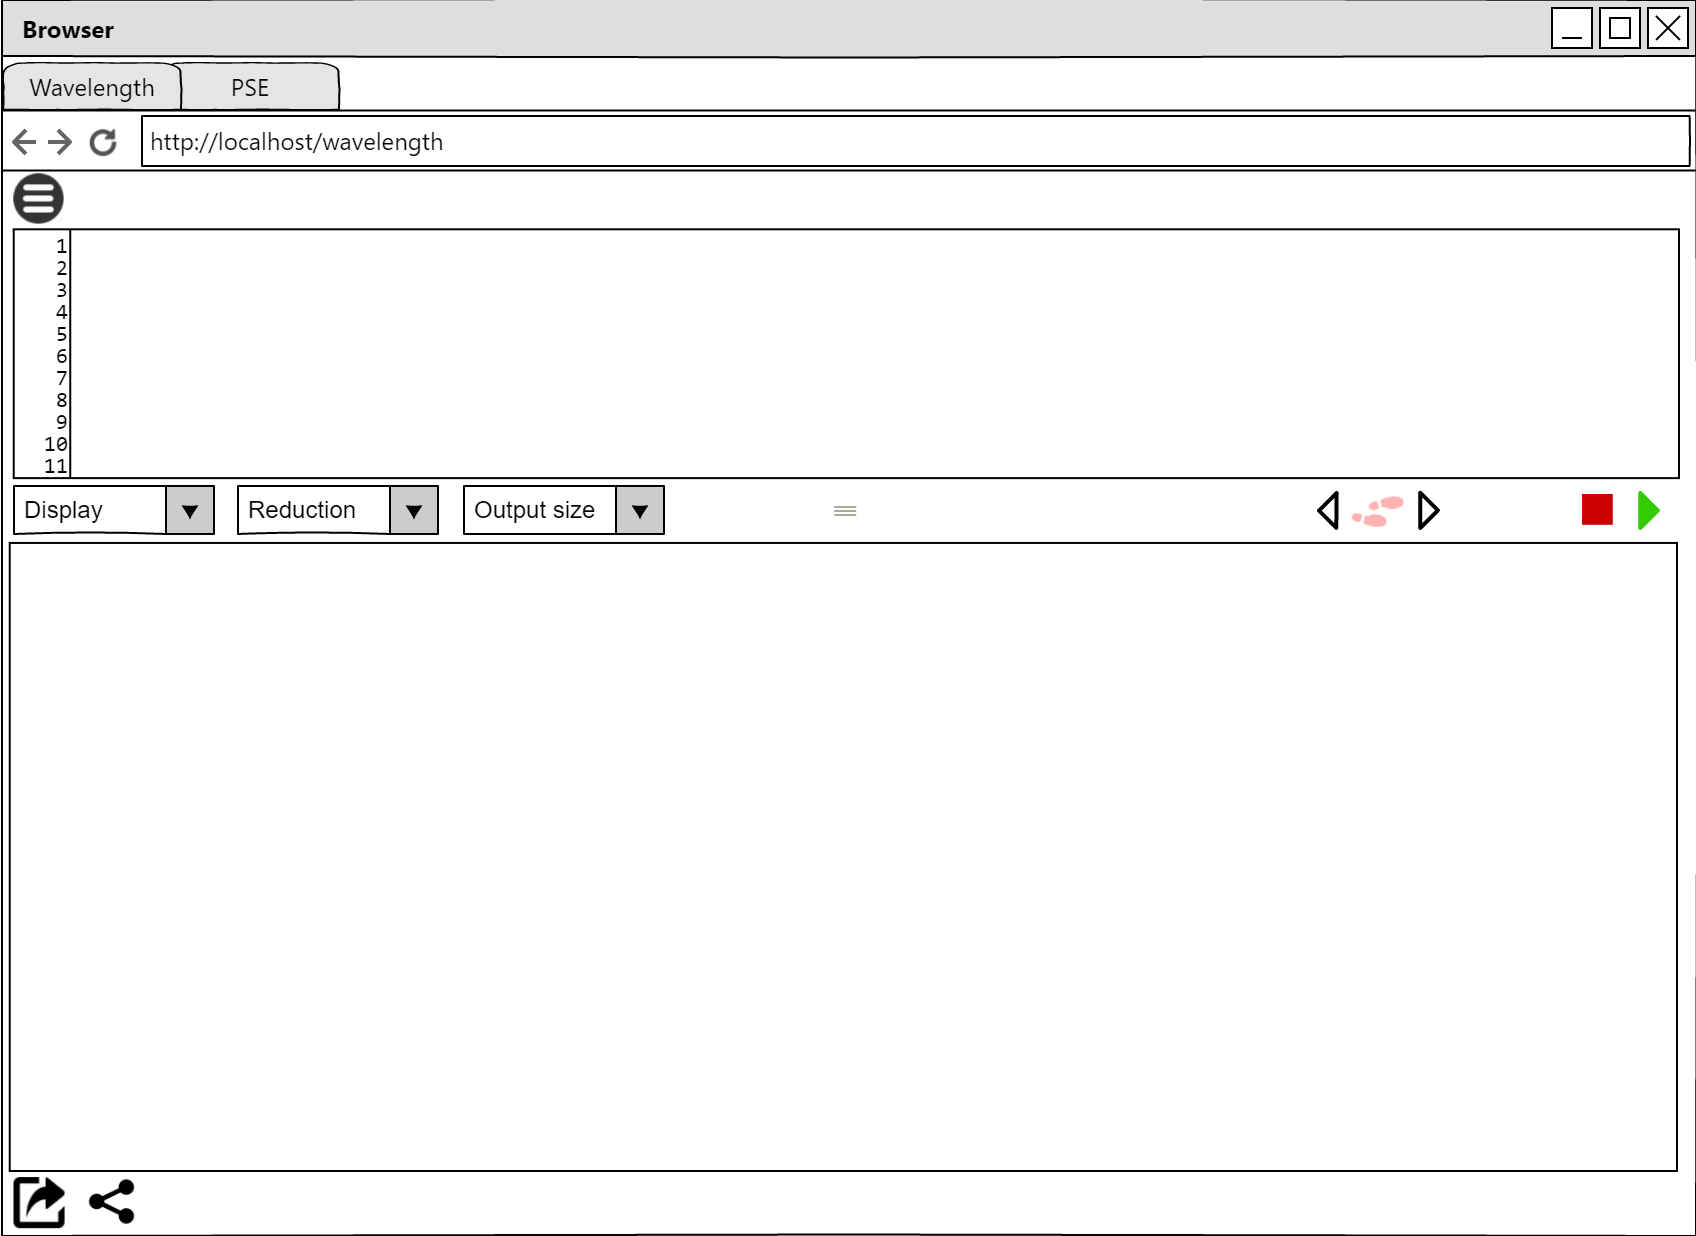
\includegraphics[width=\textwidth]{img/Startseite.png}}%lol thsi comment is important
    \only<2>{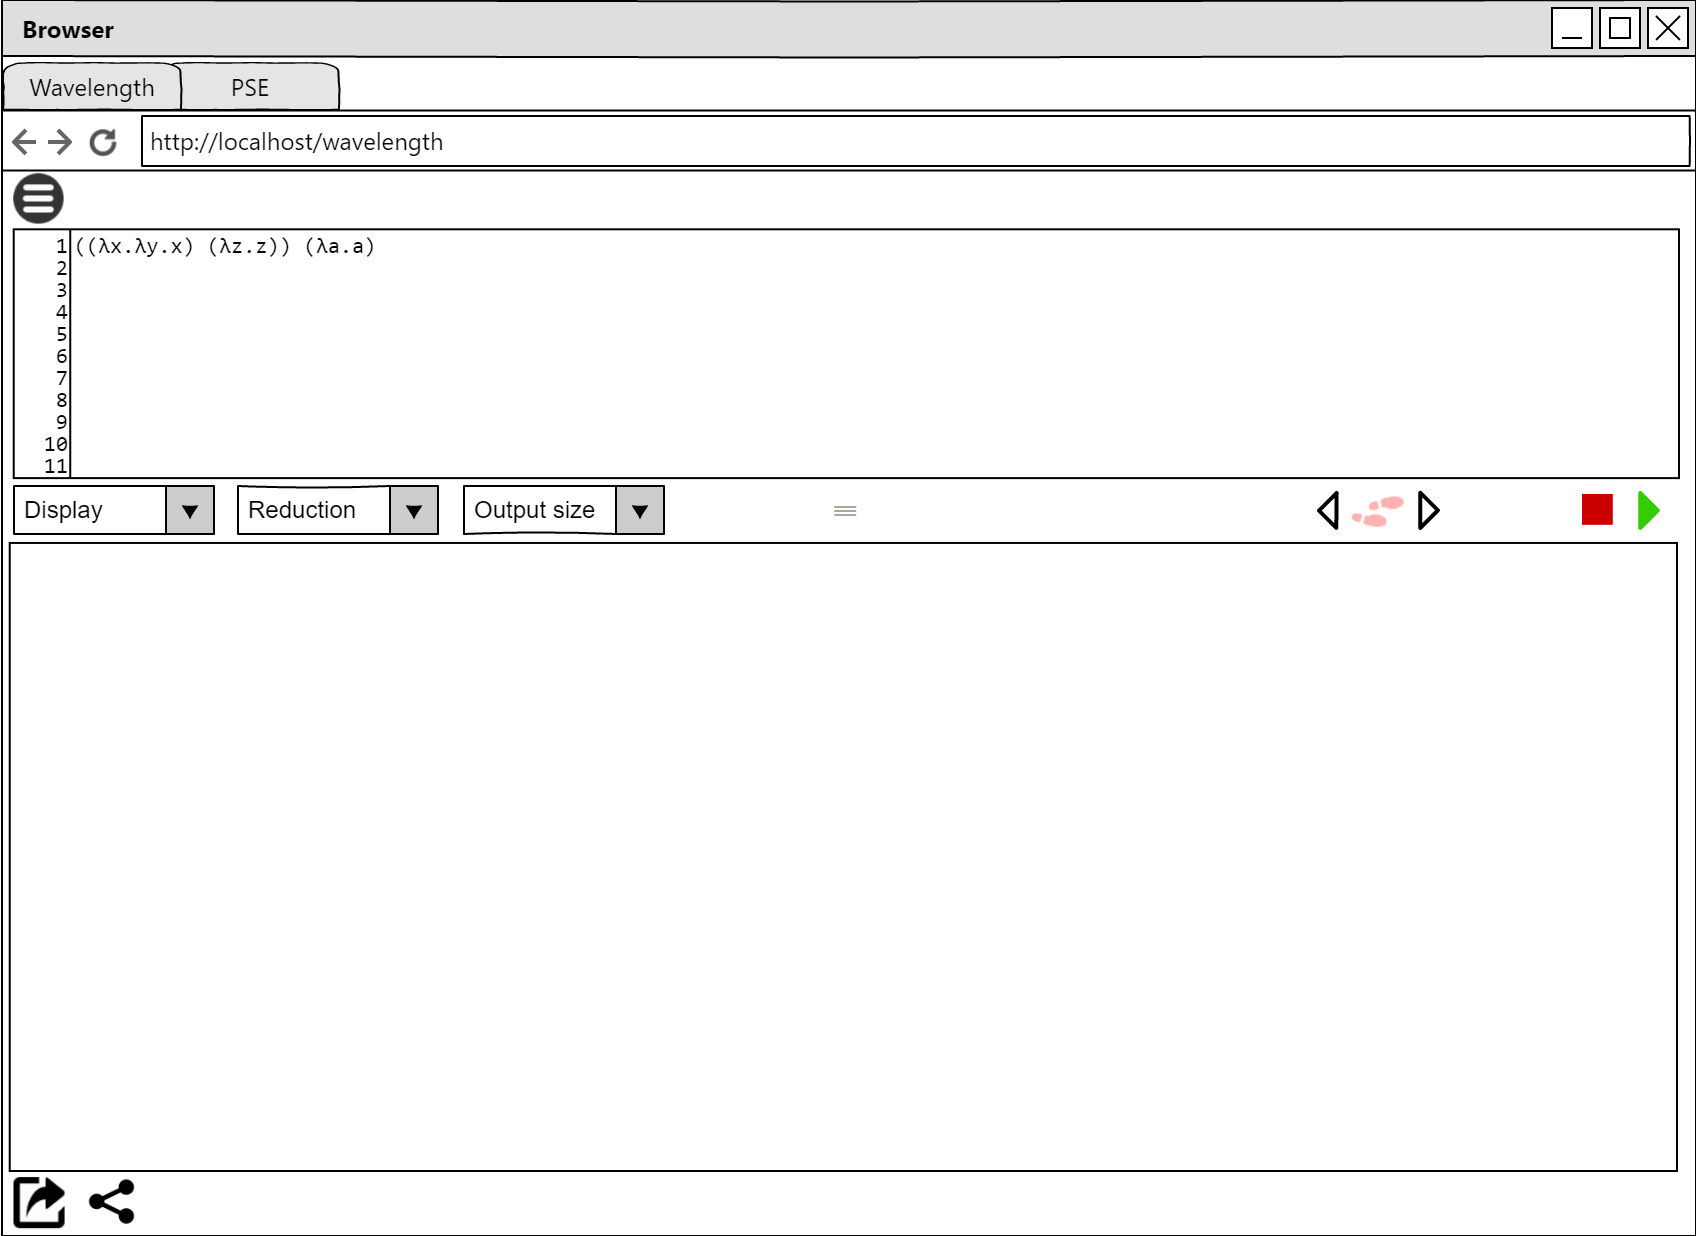
\includegraphics[width=\textwidth]{img/MussKrit_Eingabe1.png}}%
    \only<3>{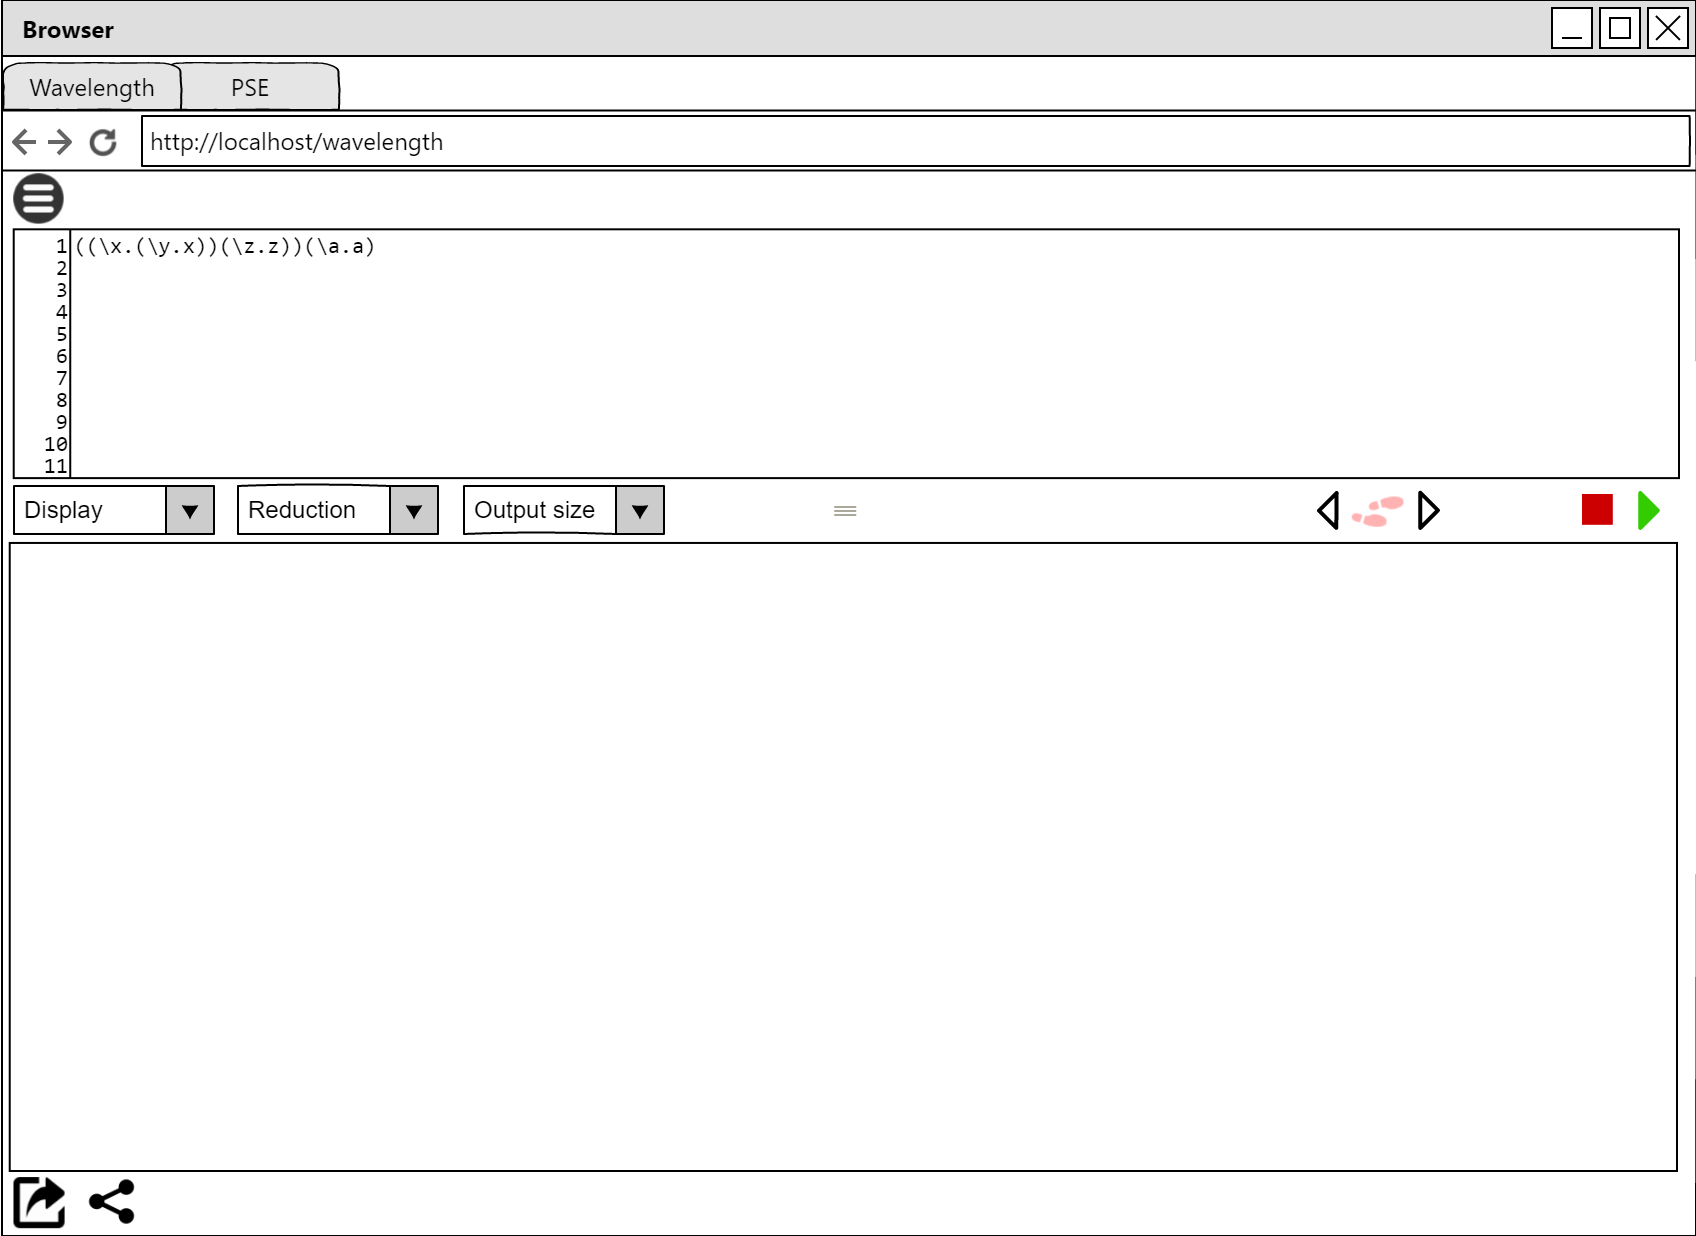
\includegraphics[width=\textwidth]{img/MussKrit_Eingabe2.png}}%
    \only<4>{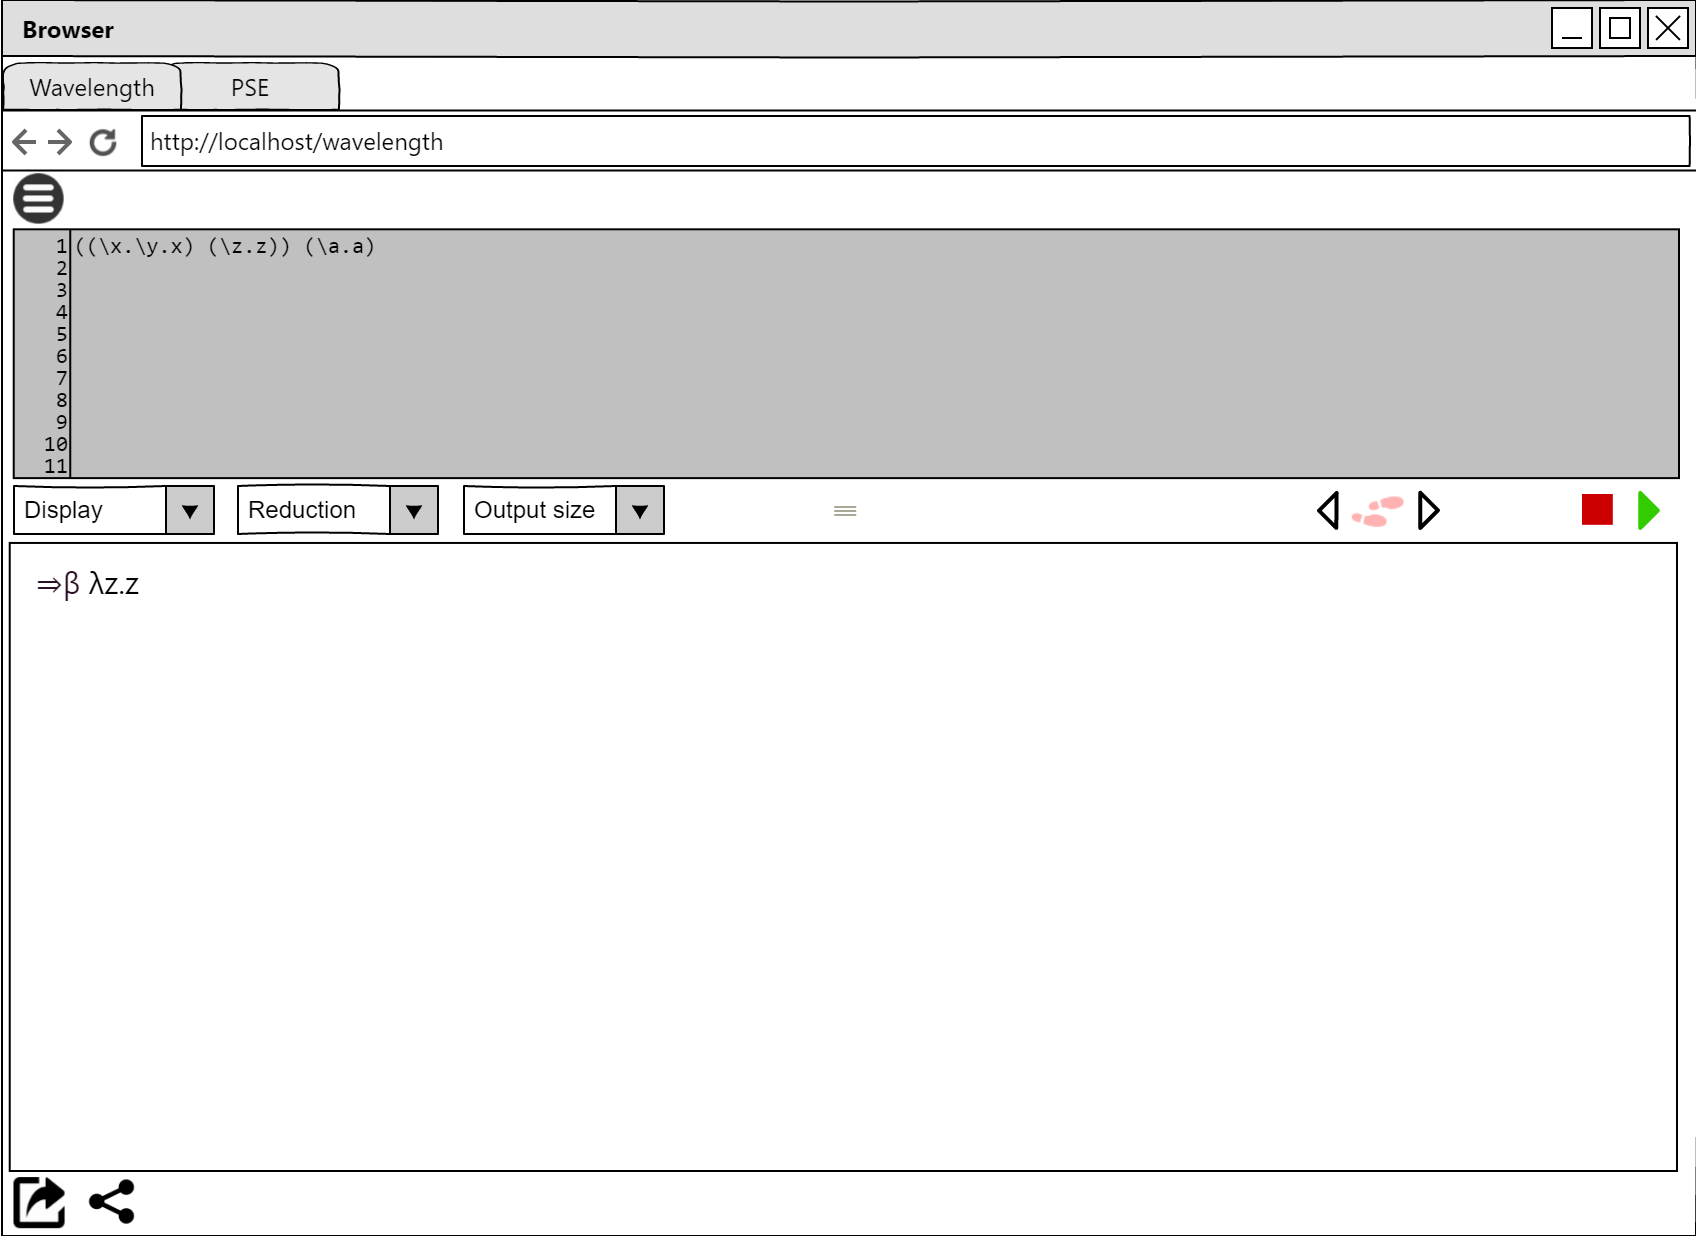
\includegraphics[width=\textwidth]{img/MussKrit_Ausgabe.png}}%
	\only<1-4>{\caption{Startseite und erste Benutzung der Entwicklungsumgebung}}
	%Voller Ausgabeumfang
    \only<5>{\includegraphics[width=\textwidth]{img/Ausgabe_FULL.png}}%
    \only<5>{\caption{Ausgabe der kompletten Auswertung}}
    %Baumdarstellung
    \only<6>{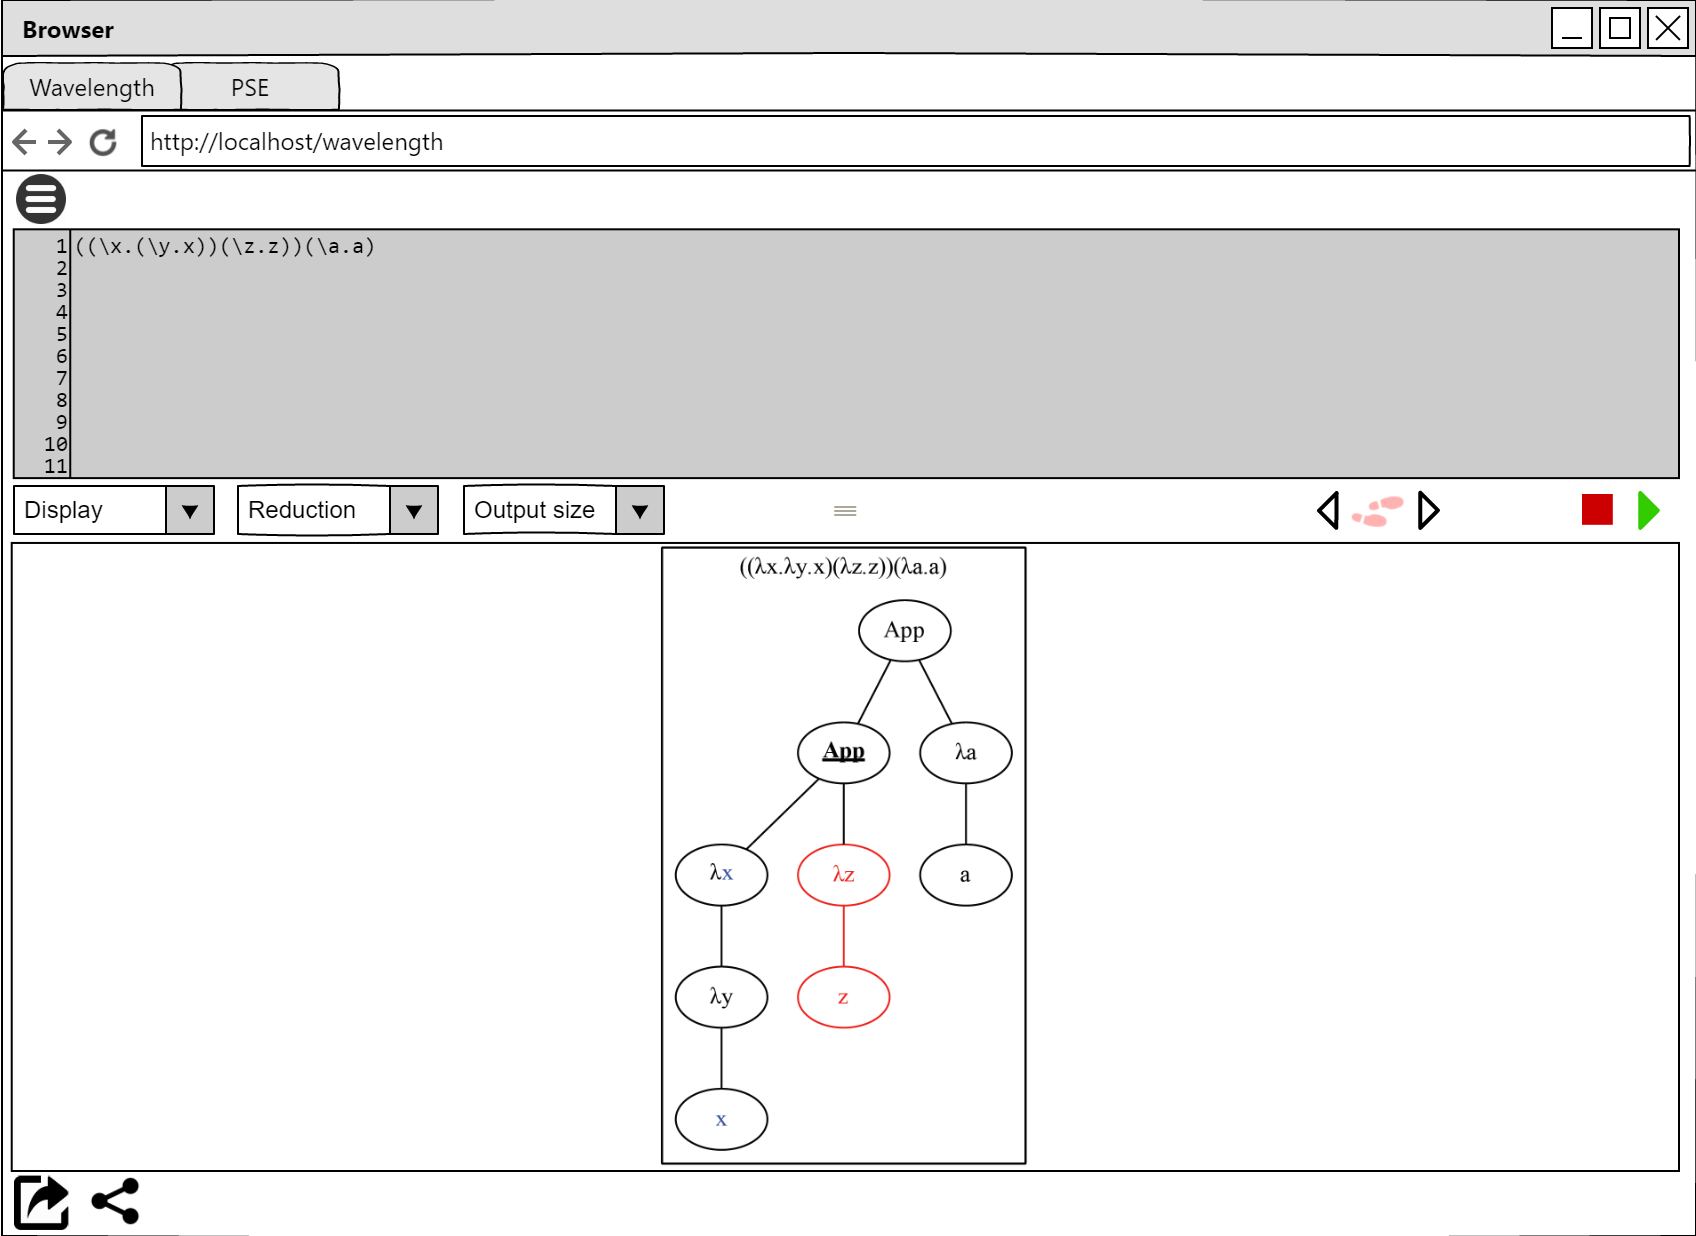
\includegraphics[width=\textwidth]{img/Ausgabe_Tree1.png}}%
    \only<7>{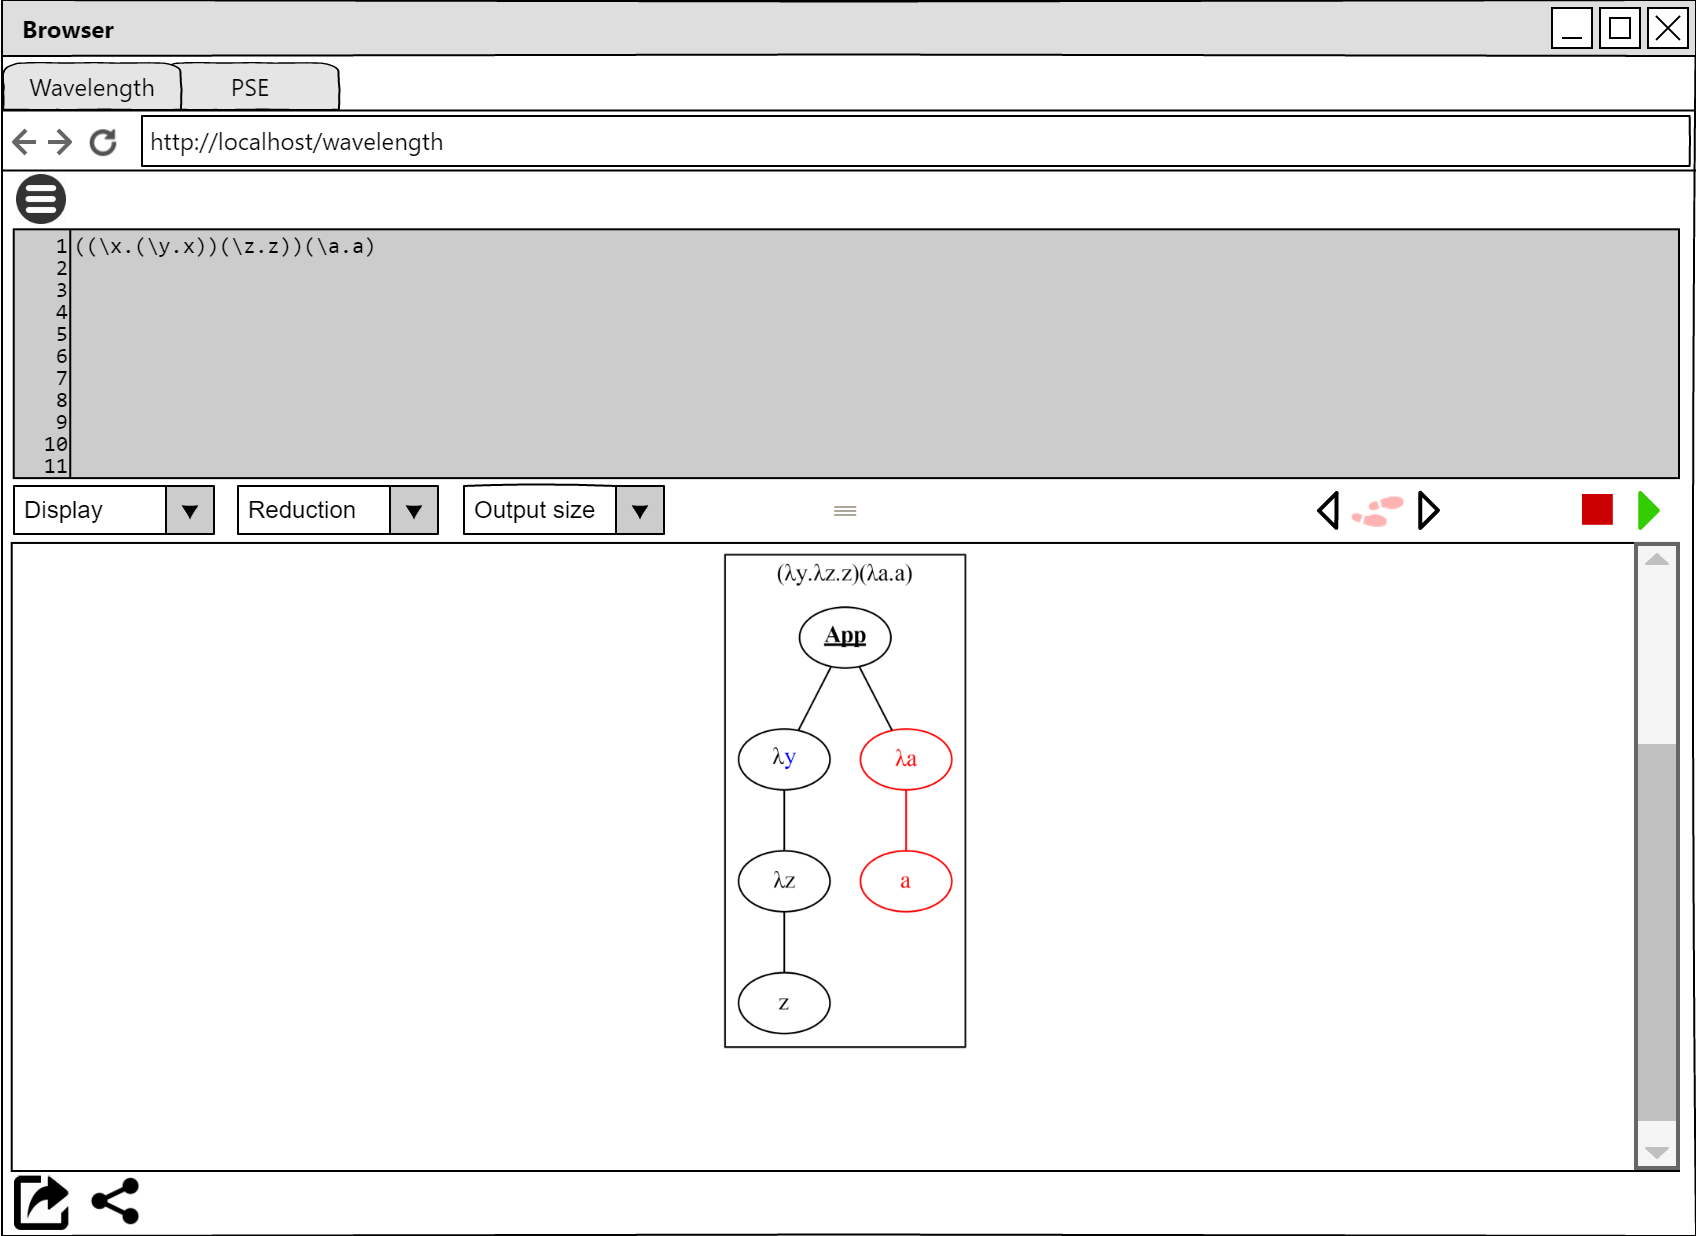
\includegraphics[width=\textwidth]{img/Ausgabe_Tree2.png}}%
    \only<8>{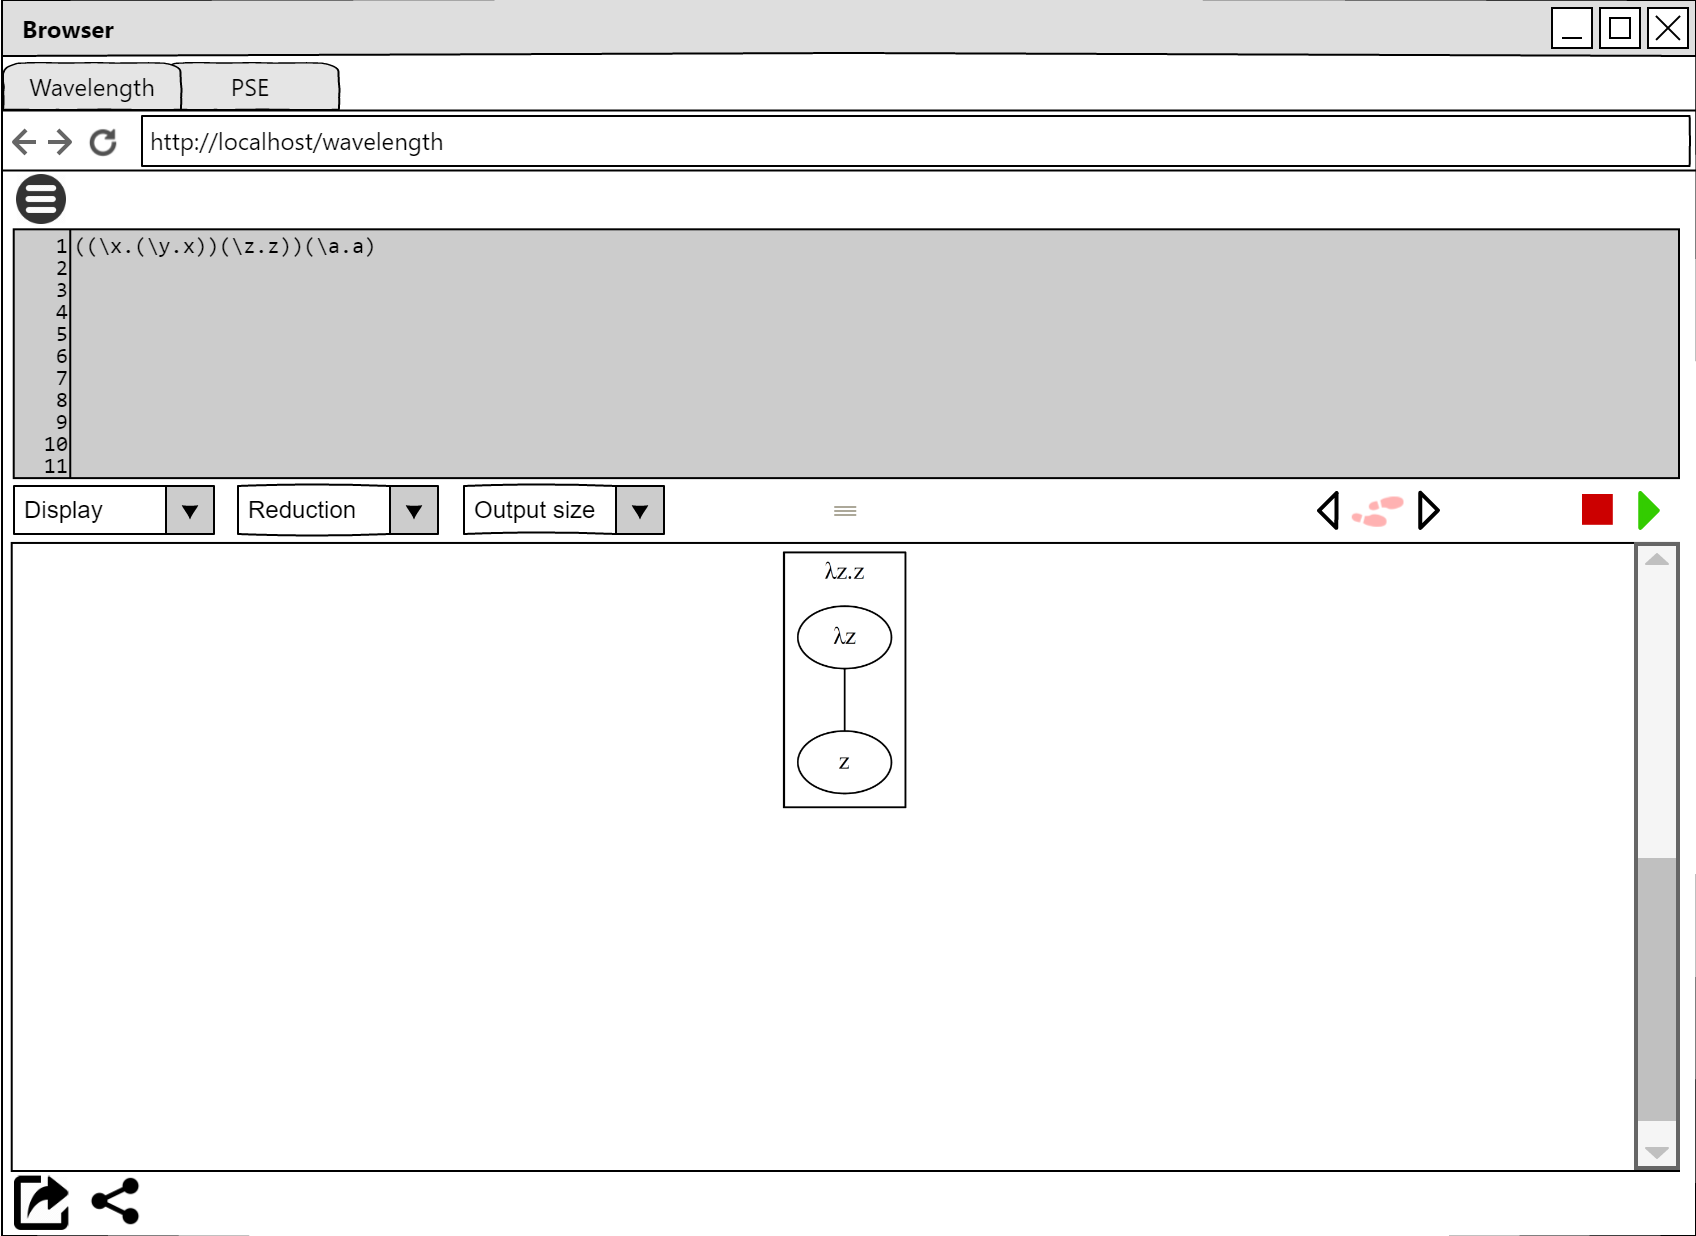
\includegraphics[width=\textwidth]{img/Ausgabe_Tree3.png}}%
    \only<6-8>{\caption{Baumdarstellung der Auswertung}}
    %Schritt-für-Schritt in Baumdarstellung
    \only<9>{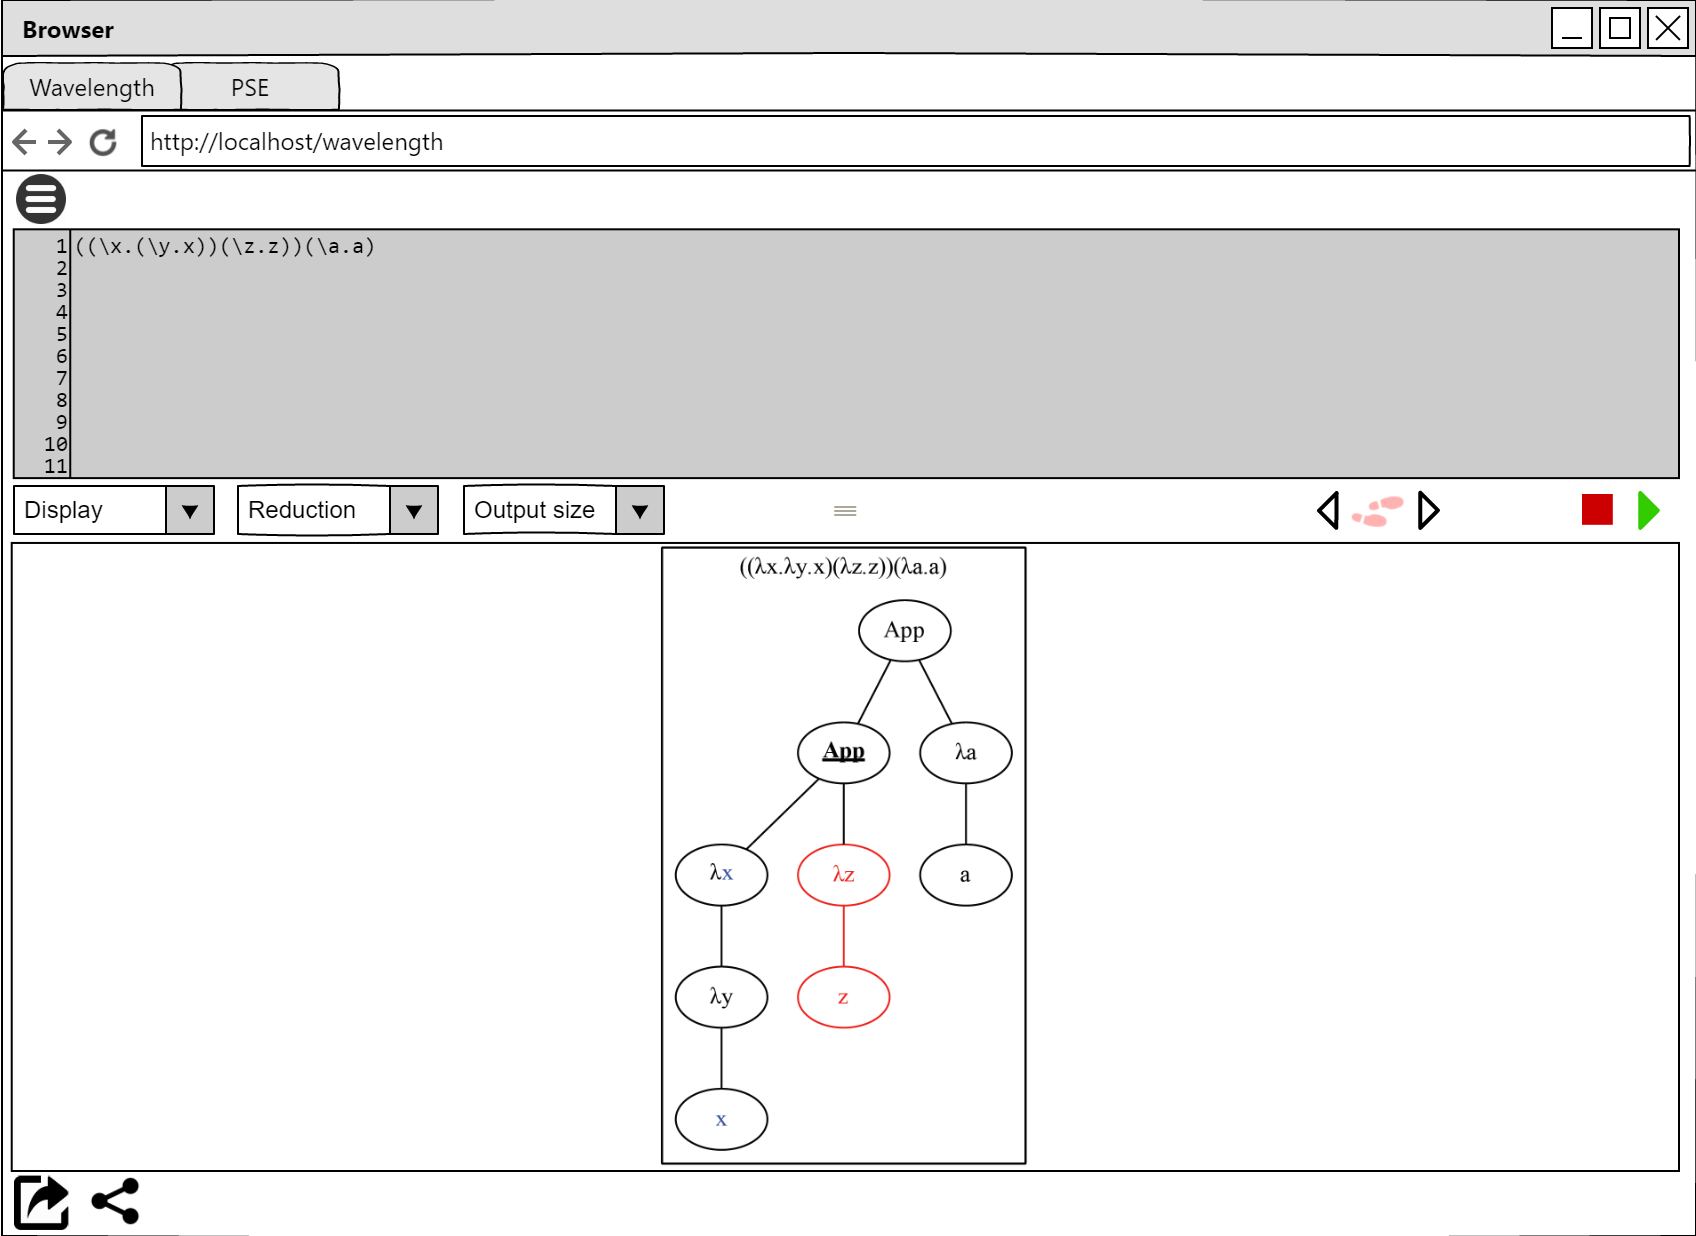
\includegraphics[width=\textwidth]{img/Ausgabe_Tree1.png}}%
    \only<10>{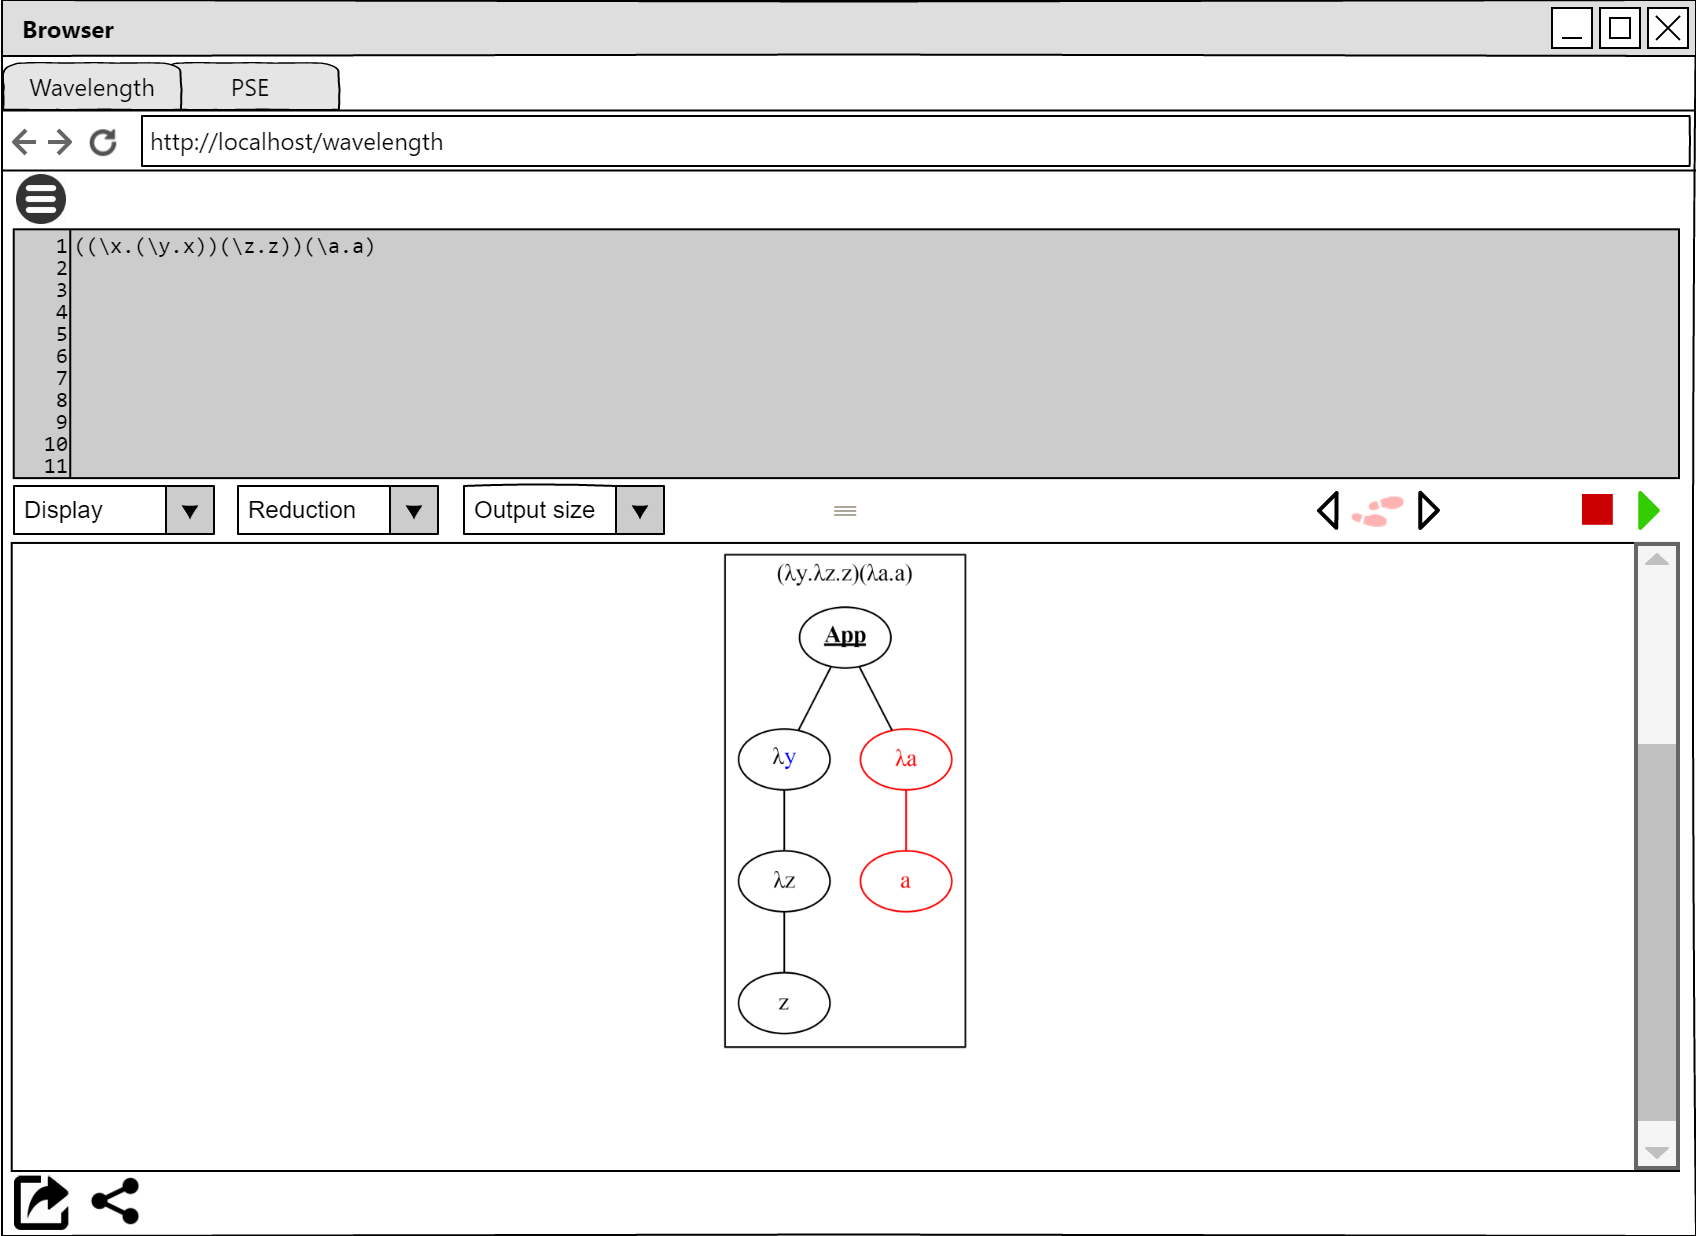
\includegraphics[width=\textwidth]{img/Ausgabe_Tree2.png}}%
    \only<11>{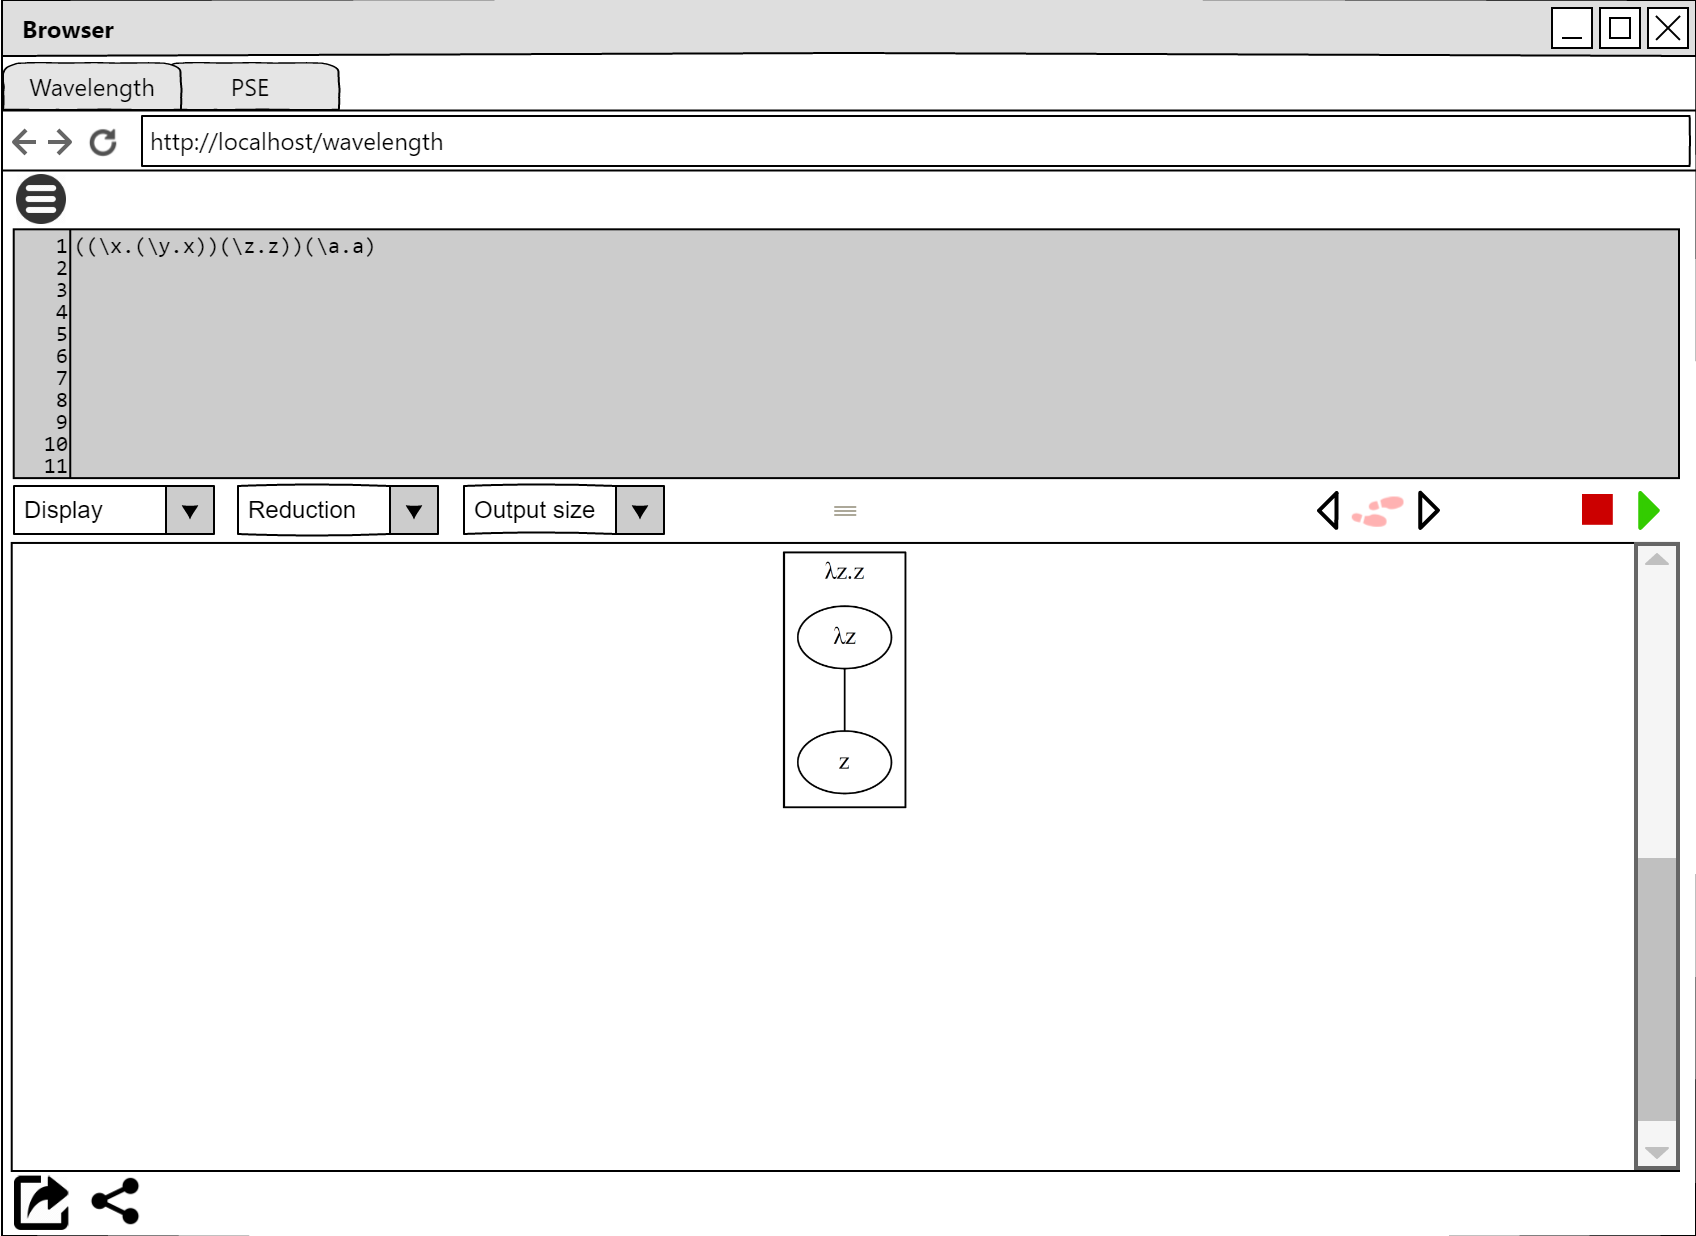
\includegraphics[width=\textwidth]{img/Ausgabe_Tree3.png}}%
    \only<9-11>{\caption{Schritt-für-Schritt Auswertung}}
    %Übungsmodus
    \only<12>{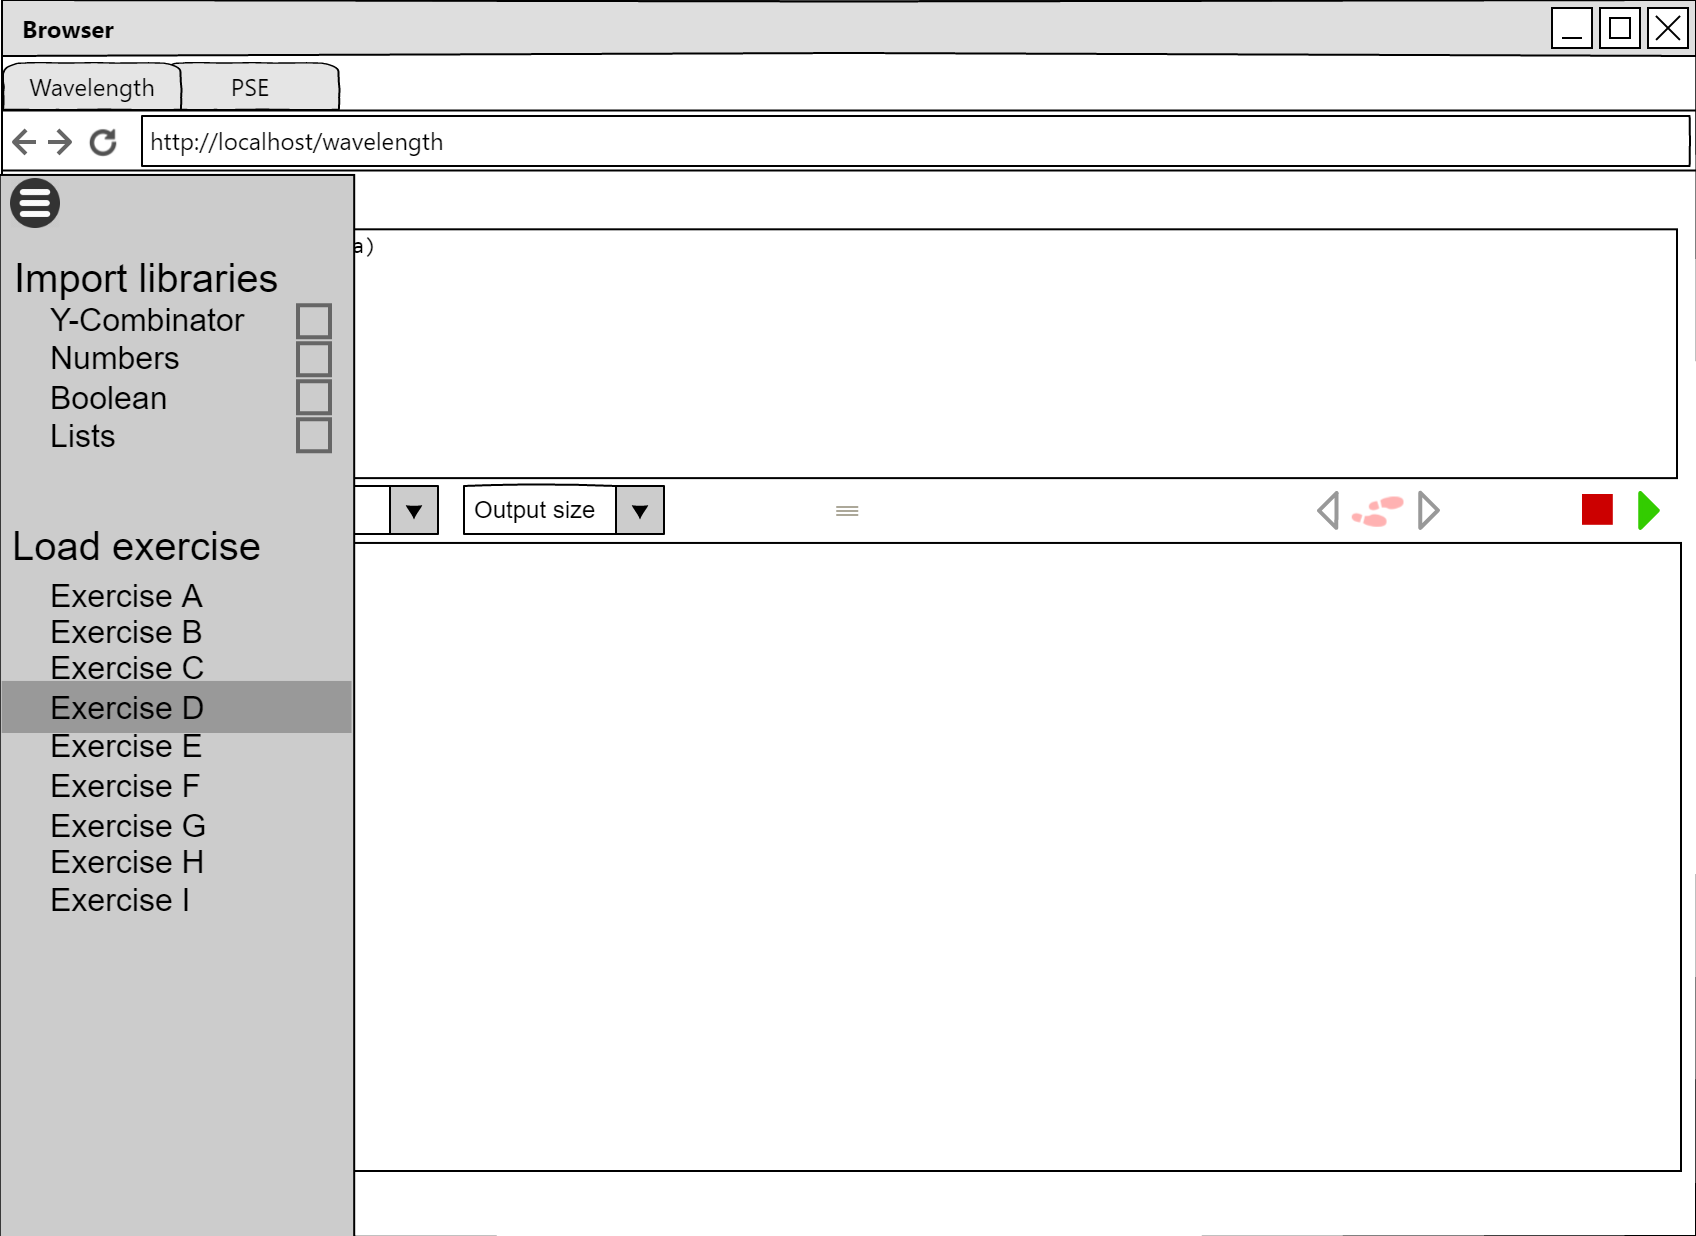
\includegraphics[width=\textwidth]{img/exercise_menue_open.png}}%
    \only<13>{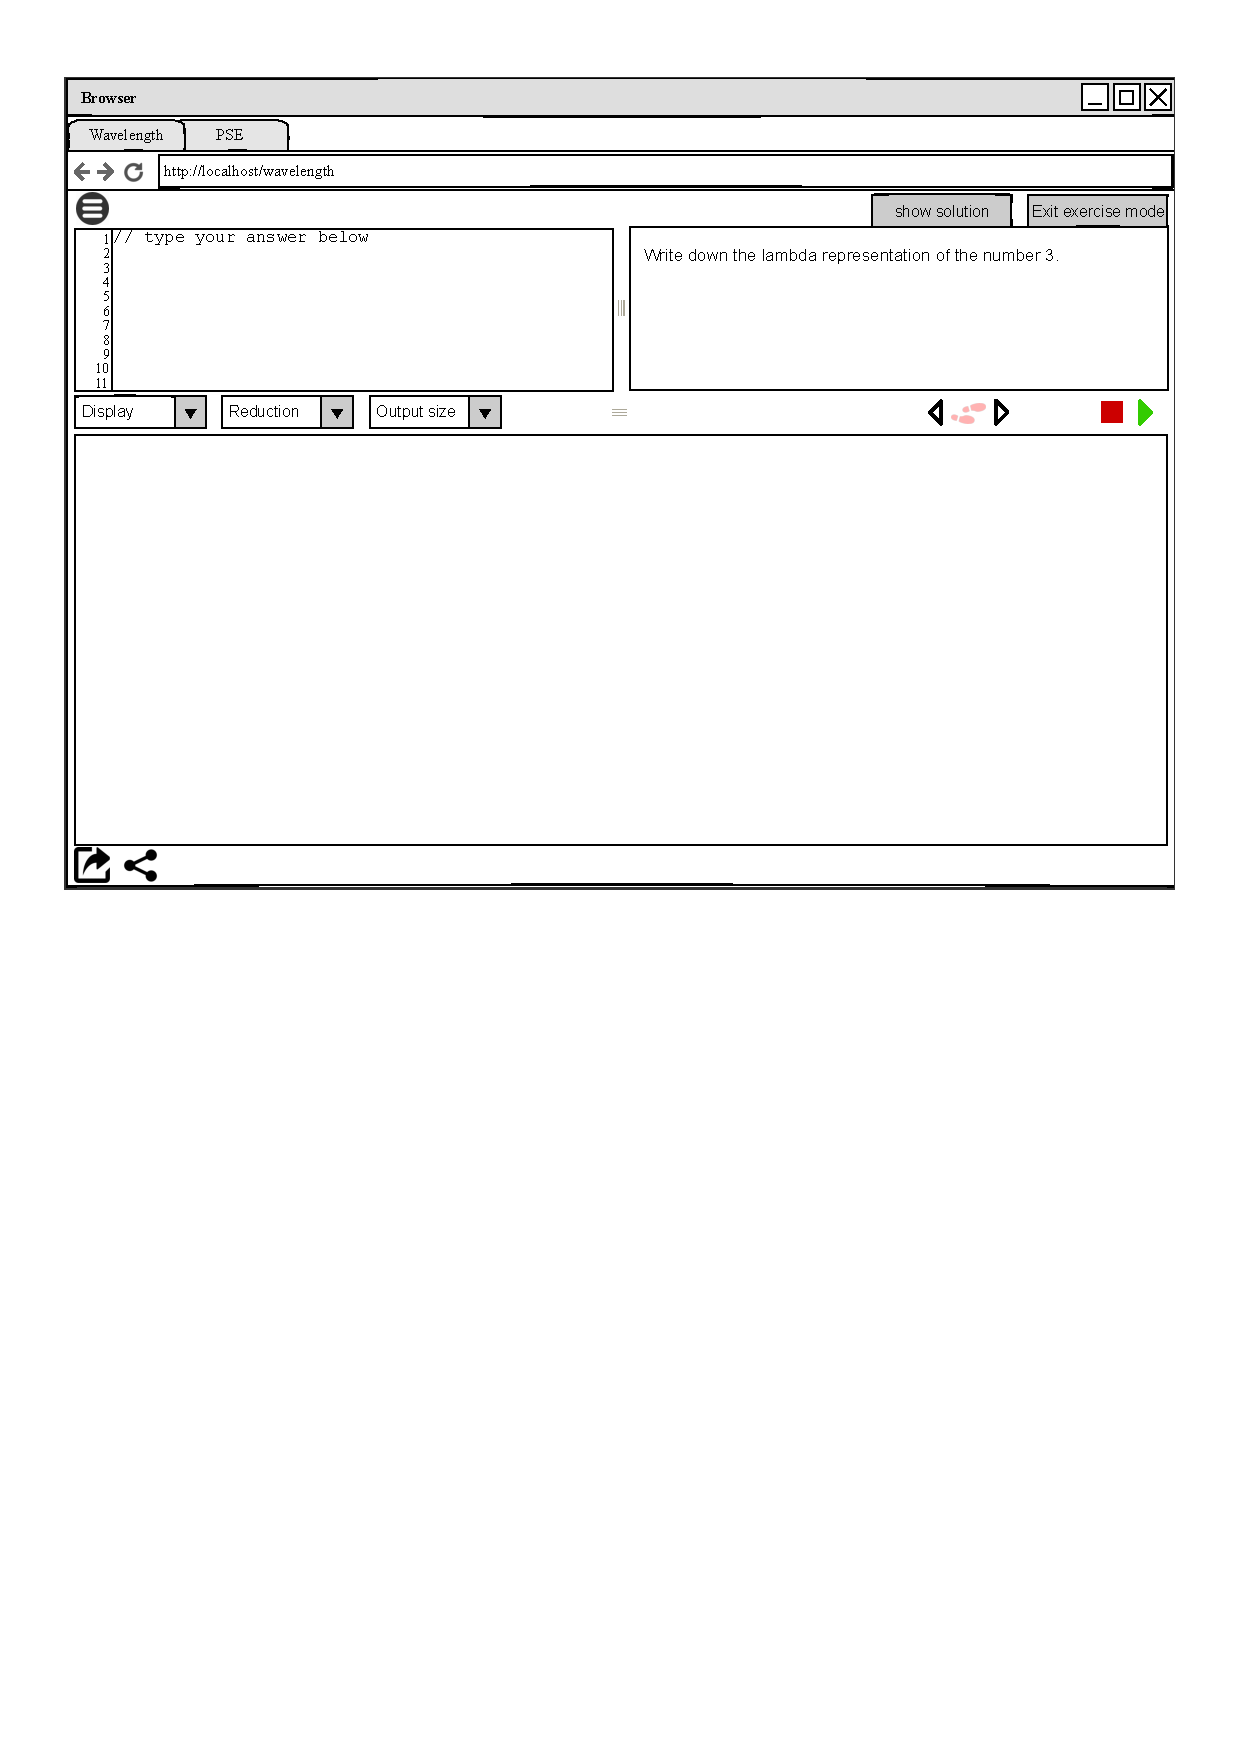
\includegraphics[width=\textwidth]{img/Exercise_(1).pdf}}%
    \only<14>{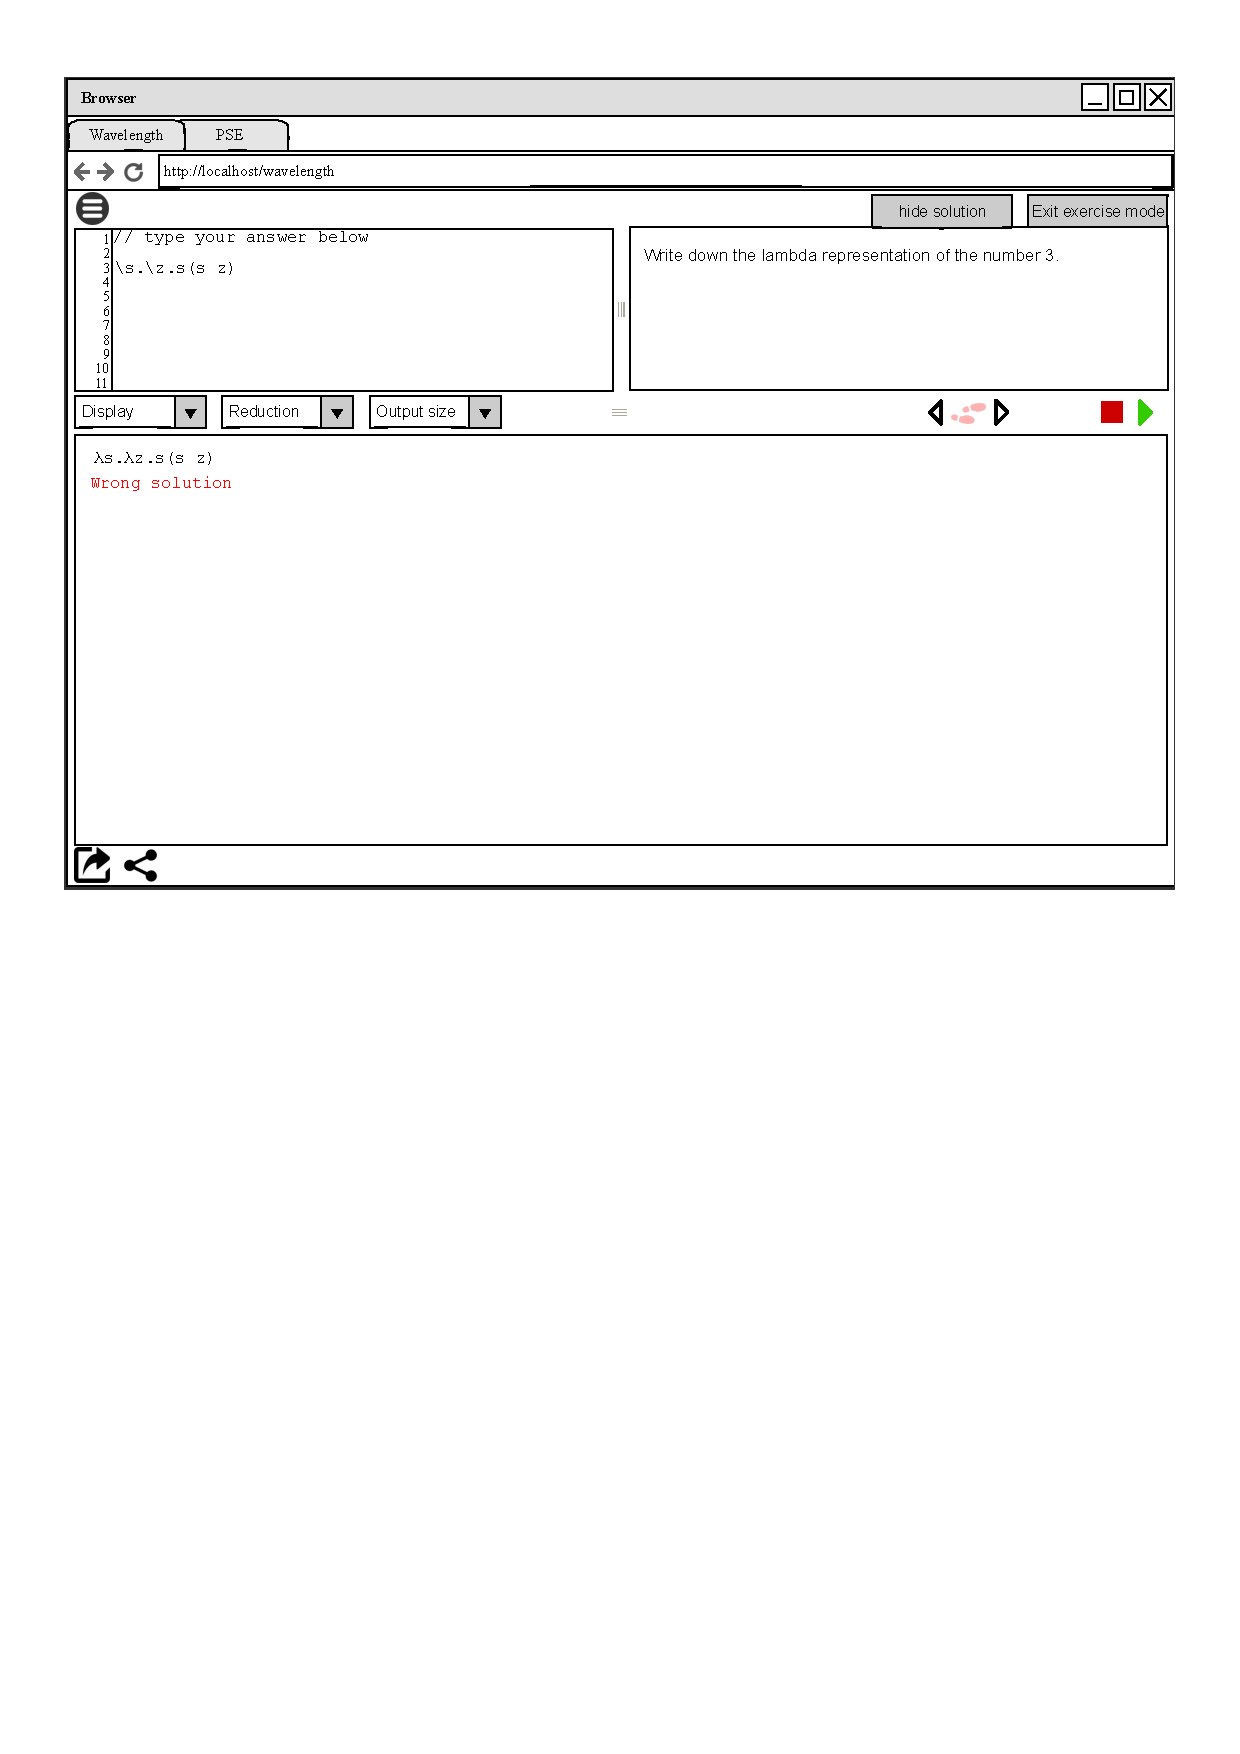
\includegraphics[width=\textwidth]{img/Exercise_(2).pdf}}%
    \only<15>{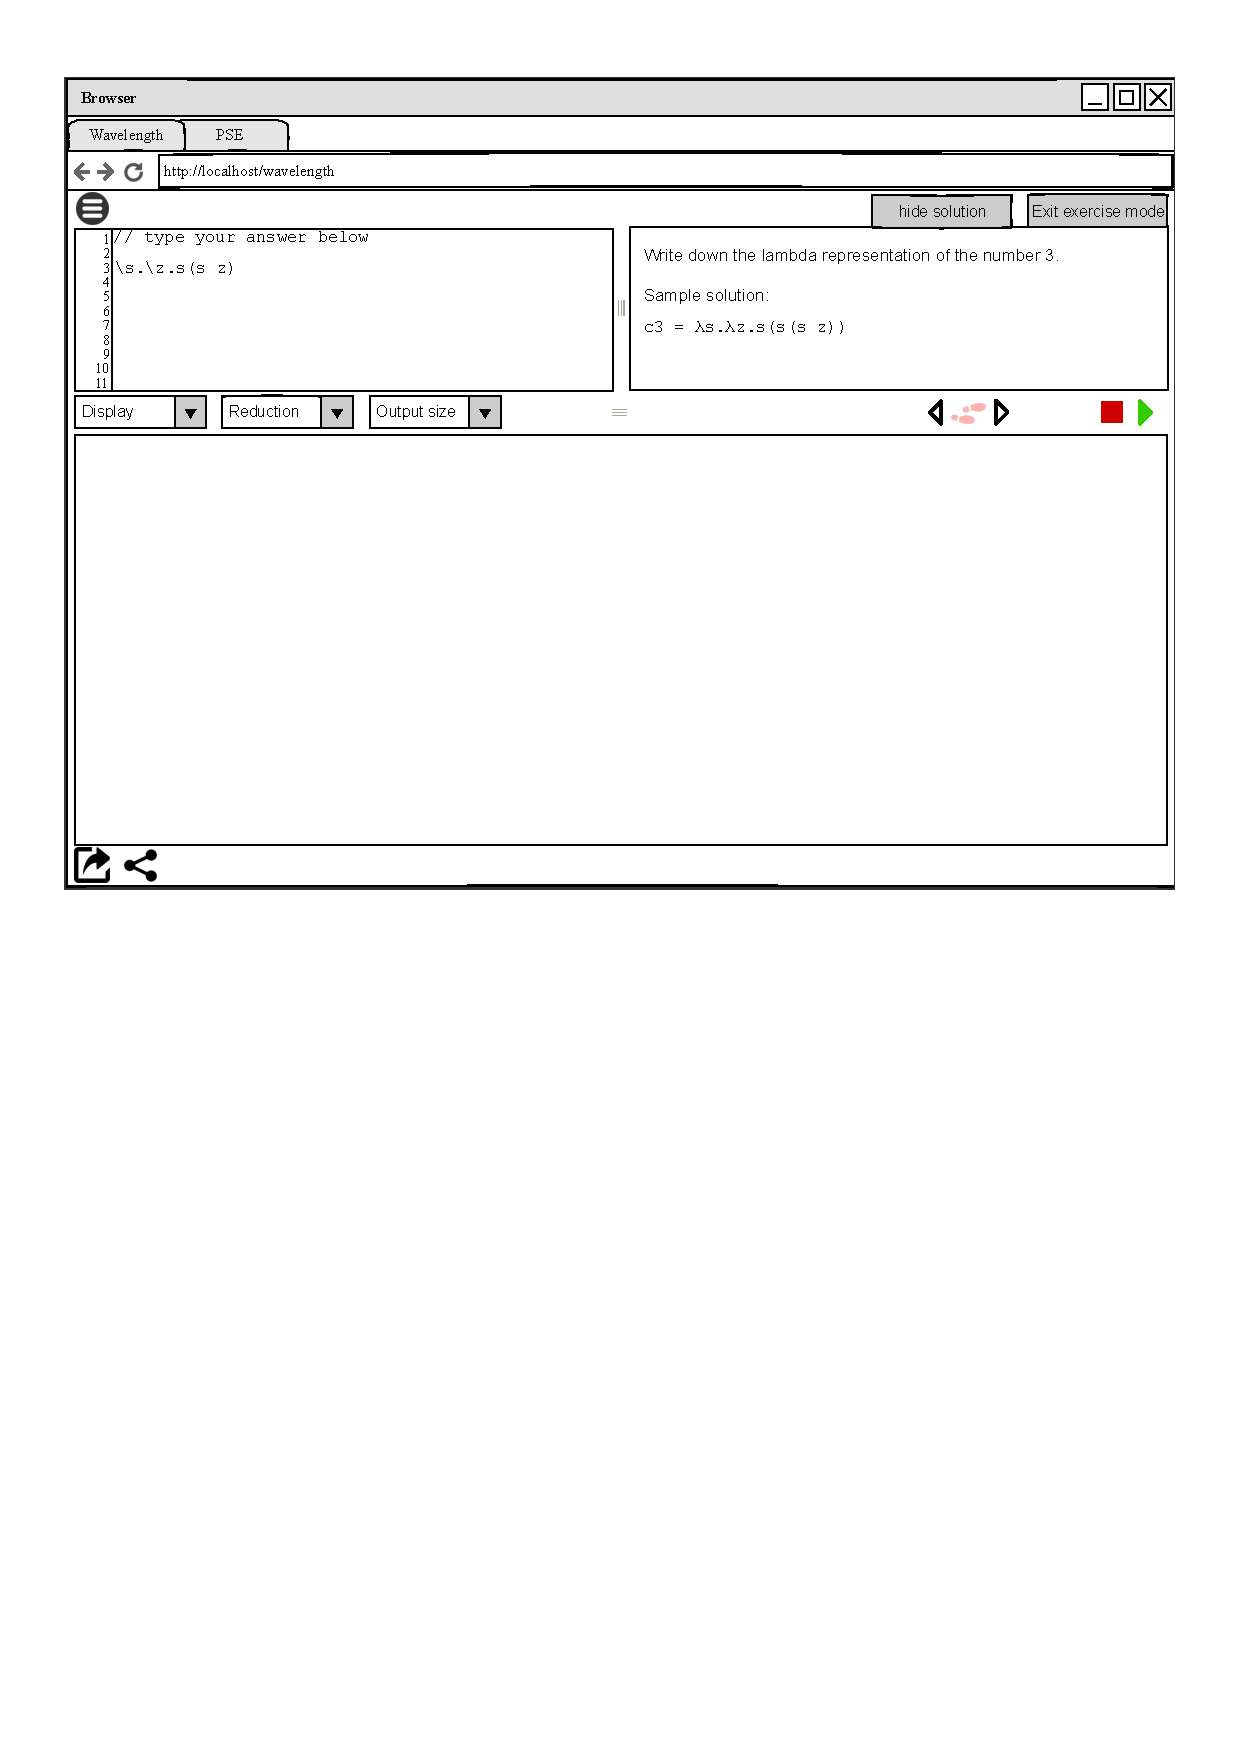
\includegraphics[width=\textwidth]{img/Exercise_(3).pdf}}%
    \only<12-15>{\caption{Übungsmodus}}
    %Fortgeschrittene Funktionen
    \only<16>{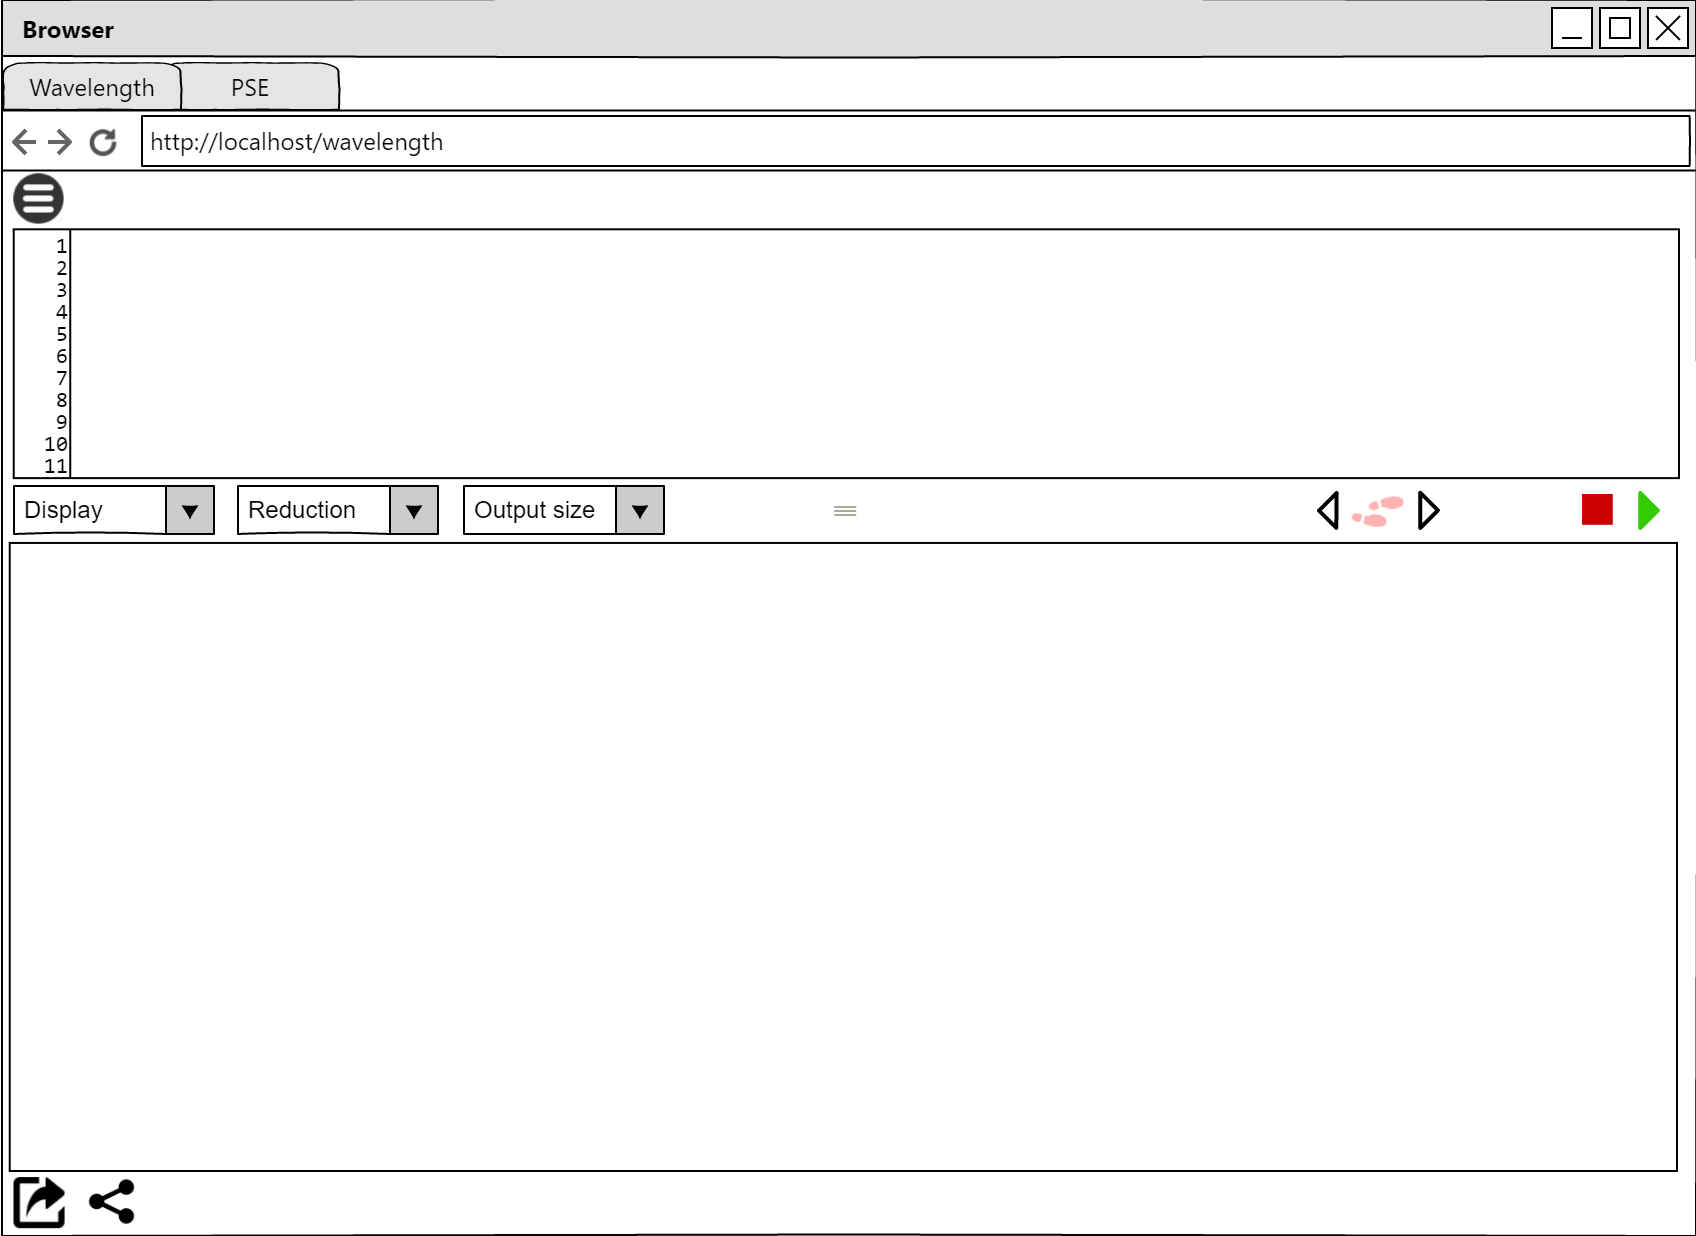
\includegraphics[width=\textwidth]{img/Startseite.png}}%
    \only<16>{\caption{Startseite der Entwicklungsumgebung}}
    \only<17>{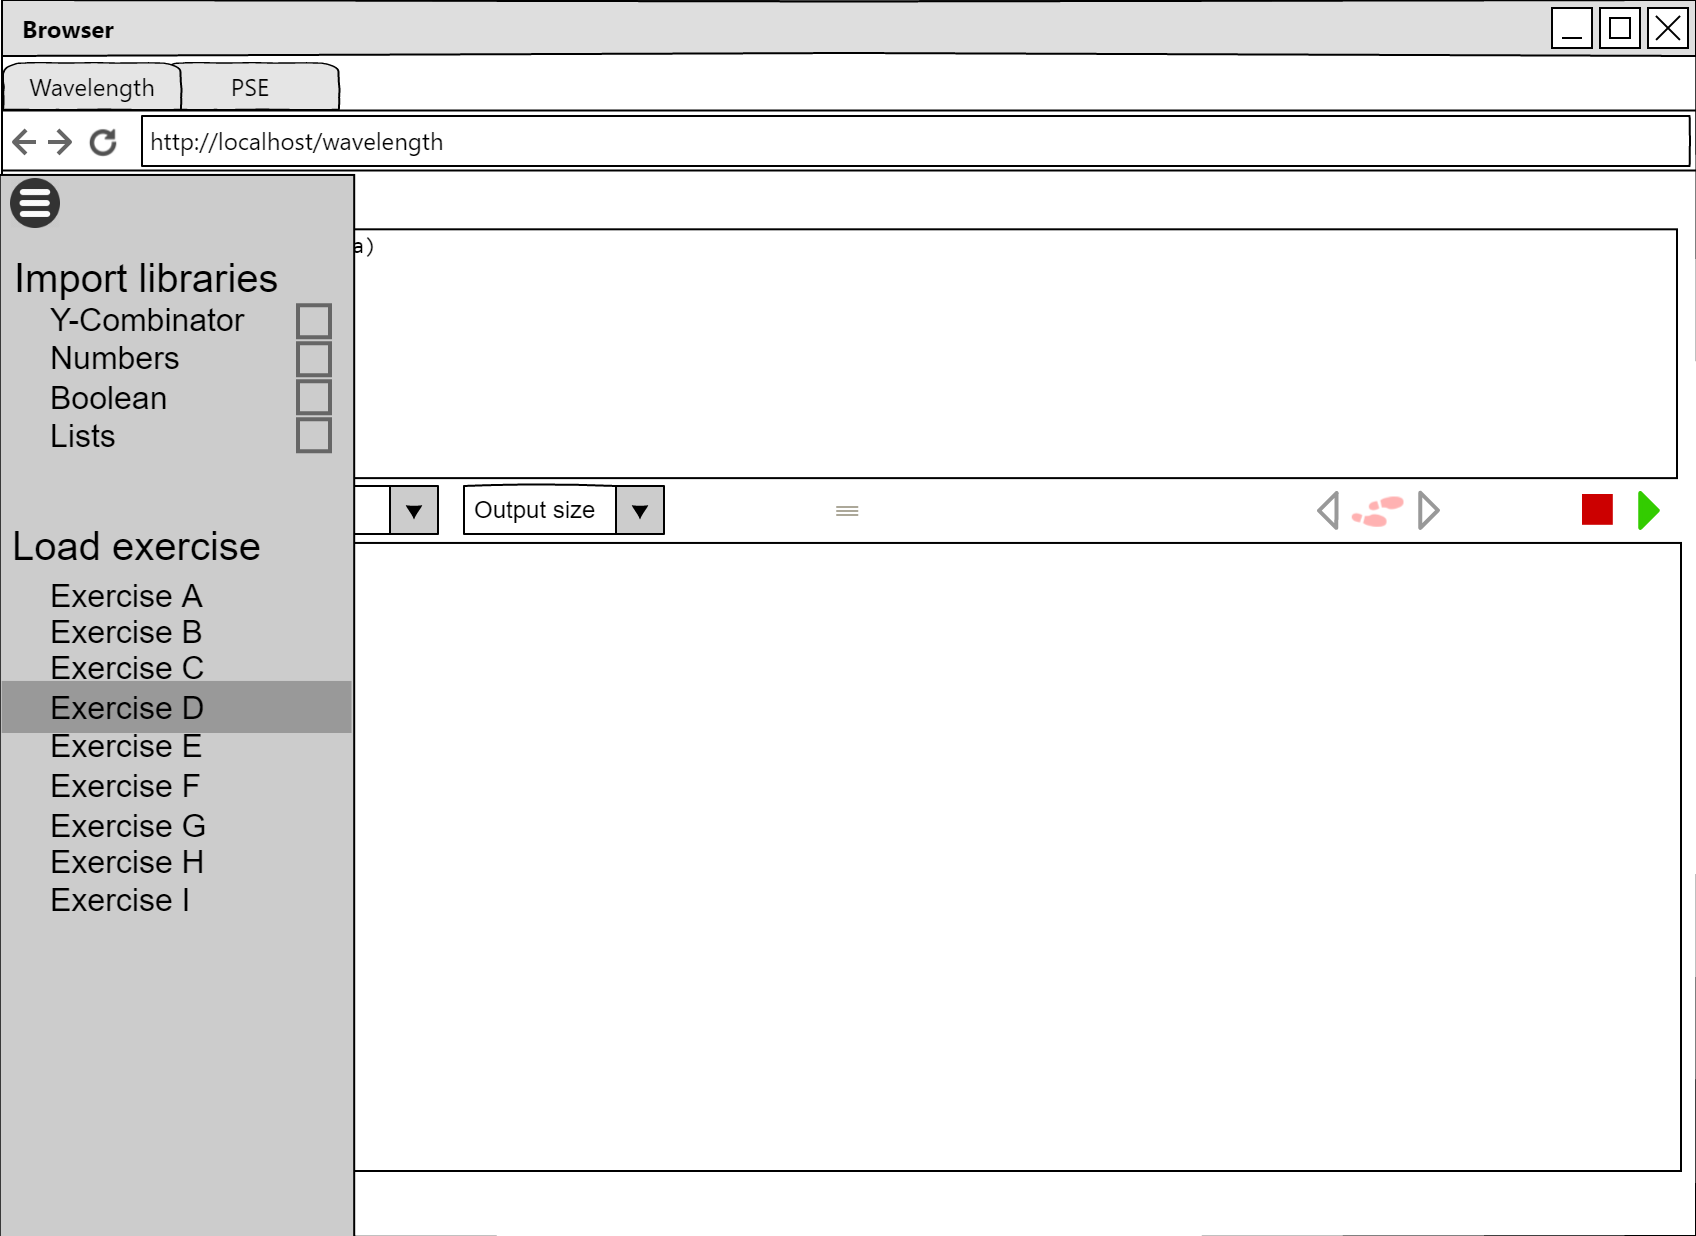
\includegraphics[width=\textwidth]{img/exercise_menue_open.png}}%
    \only<17>{\caption{Auswahl einer Bibliothek}}
    %Export von Ausgaben
    \only<18>{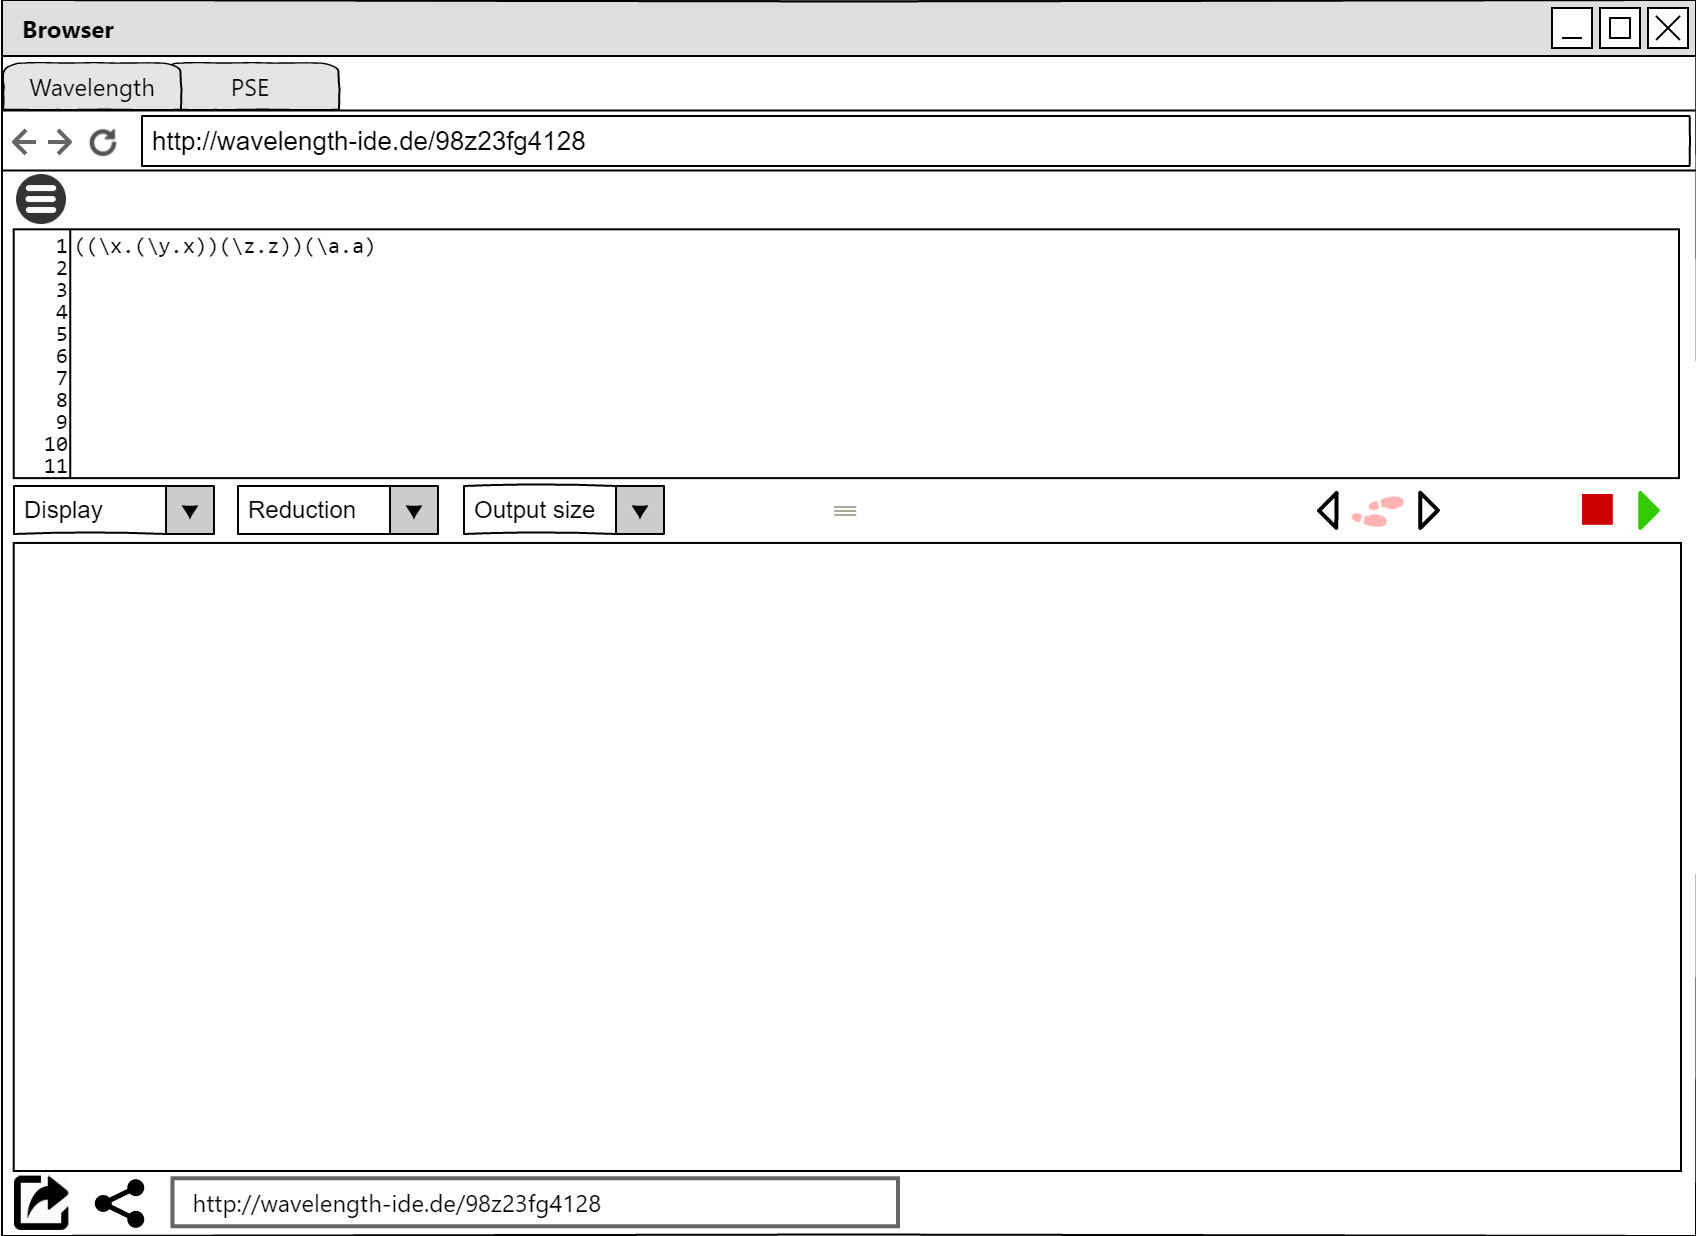
\includegraphics[width=\textwidth]{img/Share_Pressed.png}}%
    \only<19>{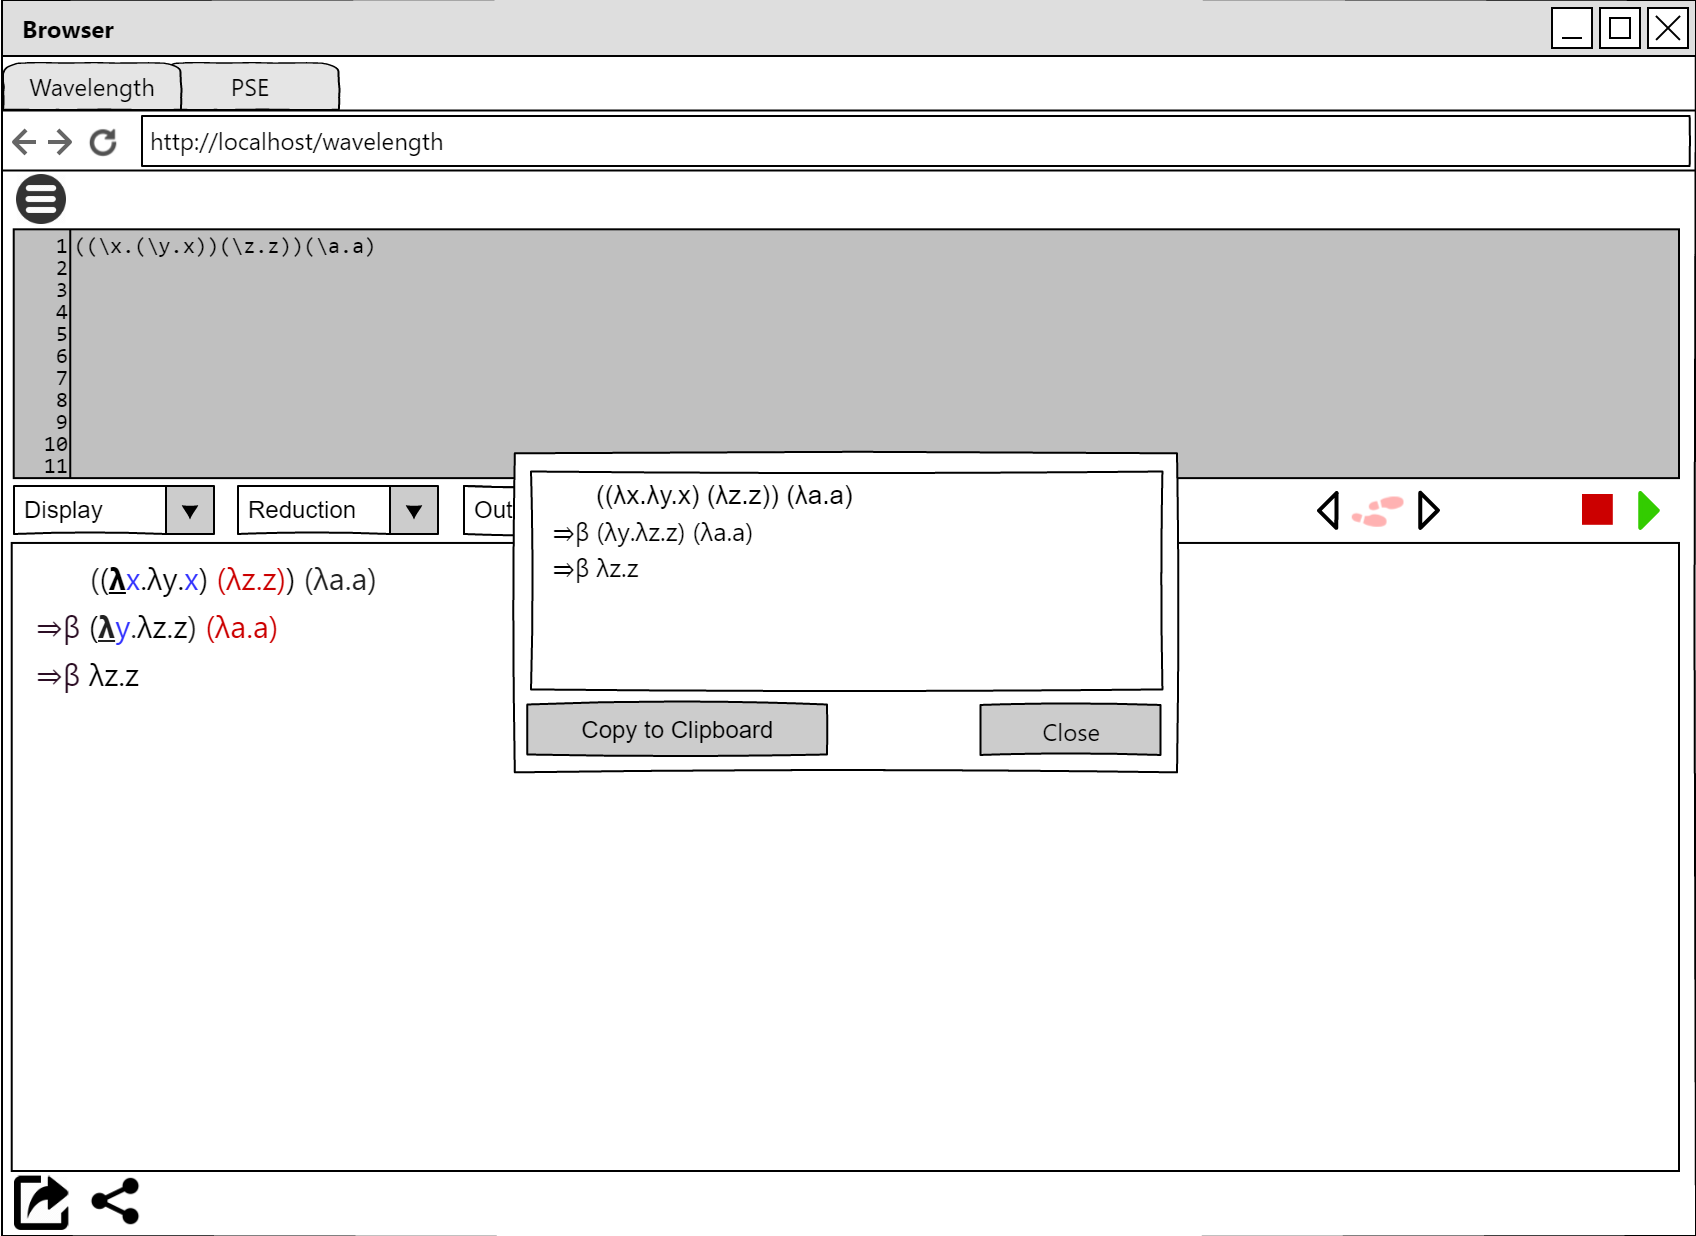
\includegraphics[width=\textwidth]{img/Share_Export.png}}%
    \only<18-19>{\caption{Teilen von $\lambda$-Auswertungen}}
\end{figure}
\end{overlayarea}

\end{frame}

\begin{frame}[noframenumbering]
  \finalpage{Vielen Dank für ihre Aufmerksamkeit!}
\end{frame}

\end{document}